%% ----------------------------------------------------------------
%% Thesis.tex -- MAIN FILE (the one that you compile with LaTeX)
%% ---------------------------------------------------------------- 

% Set up the document
\documentclass[a4paper, 12pt, oneside]{Thesis}  % Use the "Thesis" style, based on the ECS Thesis style by Steve Gunn
\graphicspath{Figures/}  % Location of the graphics files (set up for graphics to be in PDF format)

% Include any extra LaTeX packages required
\usepackage[square, numbers, comma, sort&compress]{natbib}  % Use the "Natbib" style for the references in the Bibliography
\usepackage{verbatim}  % Needed for the "comment" environment to make LaTeX comments
\usepackage{vector}  % Allows "\bvec{}" and "\buvec{}" for "blackboard" style bold vectors in maths
\hypersetup{urlcolor=blue, colorlinks=true}  % Colours hyperlinks in blue, but this can be distracting if there are many links.
\usepackage{titlesec}
\usepackage{amssymb}
\usepackage{pdflscape}
\usepackage{array}
\usepackage{longtable}
\usepackage[table]{xcolor}
\usepackage{caption}
%% -----------------Front page-------------------------------------
\begin{document}
\pagestyle{empty}
\centerline{\small{'ALEXANDRU IOAN CUZA UNIVERSITY' IA\c SI}}
\vspace{0.5cm}
\centerline{\textbf{\Large{\textsf{FACULTY OF COMPUTER SCIENCE}}}}
\vspace{3cm}
\begin{center}
	
\includegraphics[width=3cm,height=3cm]{Pictures/fii-01.png}
\end{center}
\vspace{3cm}
\centerline{\Large{MASTER THESIS}}
\vspace{1cm}
\centerline{\textbf{\LARGE{We shall see}}}
\vspace{0.2cm}
\centerline{\textbf{\LARGE{A proper title}}}
\vspace{1cm}
\centerline{proposed by}
\vspace{1cm}
\centerline{\textbf{\Large{\textsf{Radu-George Rusu}}}}
\vspace{2cm}
\centerline{\textsf{\textbf{Session:} \textit{July, 2019}}}
\vspace{0.5cm}
\centerline{Scientific coordinator}
\vspace{0.5cm}
\centerline{\textsf{\textbf{\large{???, Dr. Liviu Ciortuz}}}}

\clearpage
%% ----------------------------------------------------------------

%% --------------Page Title----------------------------------------
\pagestyle{empty}
\centerline{\textbf{\large{\textsf{ALEXANDRU IOAN CUZA UNIVERSITY IA\c SI}}}}
\vspace{0.5cm}
\centerline{\textbf{\large{\textsf{FACULTY OF COMPUTER SCIENCE}}}}
\vspace{5cm}
\centerline{\textbf{\LARGE{We shall see}}}
\vspace{0.2cm}
\centerline{\textbf{\LARGE{a proper title}}}
\vspace{3cm}
\centerline{\textbf{\Large{\textsf{Radu-George Rusu}}}}
\vspace{2cm}
\centerline{\Large{{\textsf{\textbf{Session:} \textit{July, 2019}}}}}
\vspace{4.5cm}
\centerline{\textbf{Scientific coordinator}}
\vspace{0.5cm}
\centerline{\textsf{\textbf{\large{???, Dr. Liviu Ciortuz}}}}

\clearpage
%% ----------------------------------------------------------------

\setstretch{1.3}  % It is better to have smaller font and larger line spacing than the other way round

% Define the page headers using the FancyHdr package and set up for one-sided printing
%\fancyhead{}  % Clears all page headers and footers
%\rhead{\thepage}  % Sets the right side header to show the page number
%\lhead{}  % Clears the left side page header

\pagestyle{fancy}  % Finally, use the "fancy" page style to implement the FancyHdr headers
%% ----------------------------------------------------------------
% Declaration Page required for the Thesis, your institution may give you a different text to place here

%% ----------------------------------------------------------------
% The "Funny Quote Page"
%\pagestyle{empty}  % No headers or footers for the following pages

%\null\vfill
% Now comes the "Funny Quote", written in italics
%\textit{``Write a funny quote here.''}

%\begin{flushright}
%If the quote is taken from someone, their name goes here
%\end{flushright}

%\vfill\vfill\vfill\vfill\vfill\vfill\null
%\clearpage  % Funny Quote page ended, start a new page
%% ----------------------------------------------------------------

% The Abstract Page
%\addtotoc{Abstract}  % Add the "Abstract" page entry to the Contents
%\abstract{
%\addtocontents{toc}{\vspace{1em}}  % Add a gap in the Contents, for aesthetics

%The Thesis Abstract is written here (and usually kept to just %this page). The page is kept centered vertically so can %expand into the blank space above the title too\ldots

%}

%\clearpage  % Abstract ended, start a new page
%% ----------------------------------------------------------------

%\setstretch{1.3}  % Reset the line-spacing to 1.3 for body text (if it has changed)

% The Acknowledgements page, for thanking everyone
%\acknowledgements{
%\addtocontents{toc}{\vspace{1em}}  % Add a gap in the Contents, for aesthetics

%The acknowledgements and the people to thank go here, don't forget to include your project advisor\ldots

%}
%\clearpage  % End of the Acknowledgements
%% ----------------------------------------------------------------

\pagestyle{empty}  %The page style headers have been "empty" all this time, now use the "fancy" headers as defined before to bring them back


%% ----------------------------------------------------------------
%\lhead{An evaluation method for team project based learning}  % Set the left side page header to "Contents"
%\rhead{Radu-George Rusu}
%\cfoot{}
\pagenumbering{gobble}
\tableofcontents  % Write out the Table of Contents

%% ----------------------------------------------------------------
%\lhead{\emph{List of Figures}}  % Set the left side page header to "List if Figures"
%\listoffigures  % Write out the List of Figures

%% ----------------------------------------------------------------
%\lhead{\emph{List of Tables}}  % Set the left side page header to "List of Tables"
%\listoftables  % Write out the List of Tables

\addtocontents{toc}{\vspace{2em}}  % Add a gap in the Contents, for aesthetics


%% ----------------------------------------------------------------
\mainmatter	  % Begin normal, numeric (1,2,3...) page numbering
\pagestyle{fancy}  % Return 
\cfoot{\thepage}
% Include the chapters of the thesis, as separate files
% Just uncomment the lines as you write the chapters

\chapter*{Introduction}
%\lhead{Introduction}
%\rhead{Radu-George Rusu}
\addcontentsline{toc}{chapter}{Introduction}
Intro \cite{borda}

 % Variable Selection

\chapter{Airbus Ship Detection Challenge}
\lhead{Airbus Ship Detection Challenge}
\rhead{Radu-George Rusu}
\label{DatasetChapter}

This chapter presents the data set used for the experiment in this paper, the Kaggle competition that it was used in, and an analysis over how the data looks and can impact the experiments.

\begin{figure}[H]
	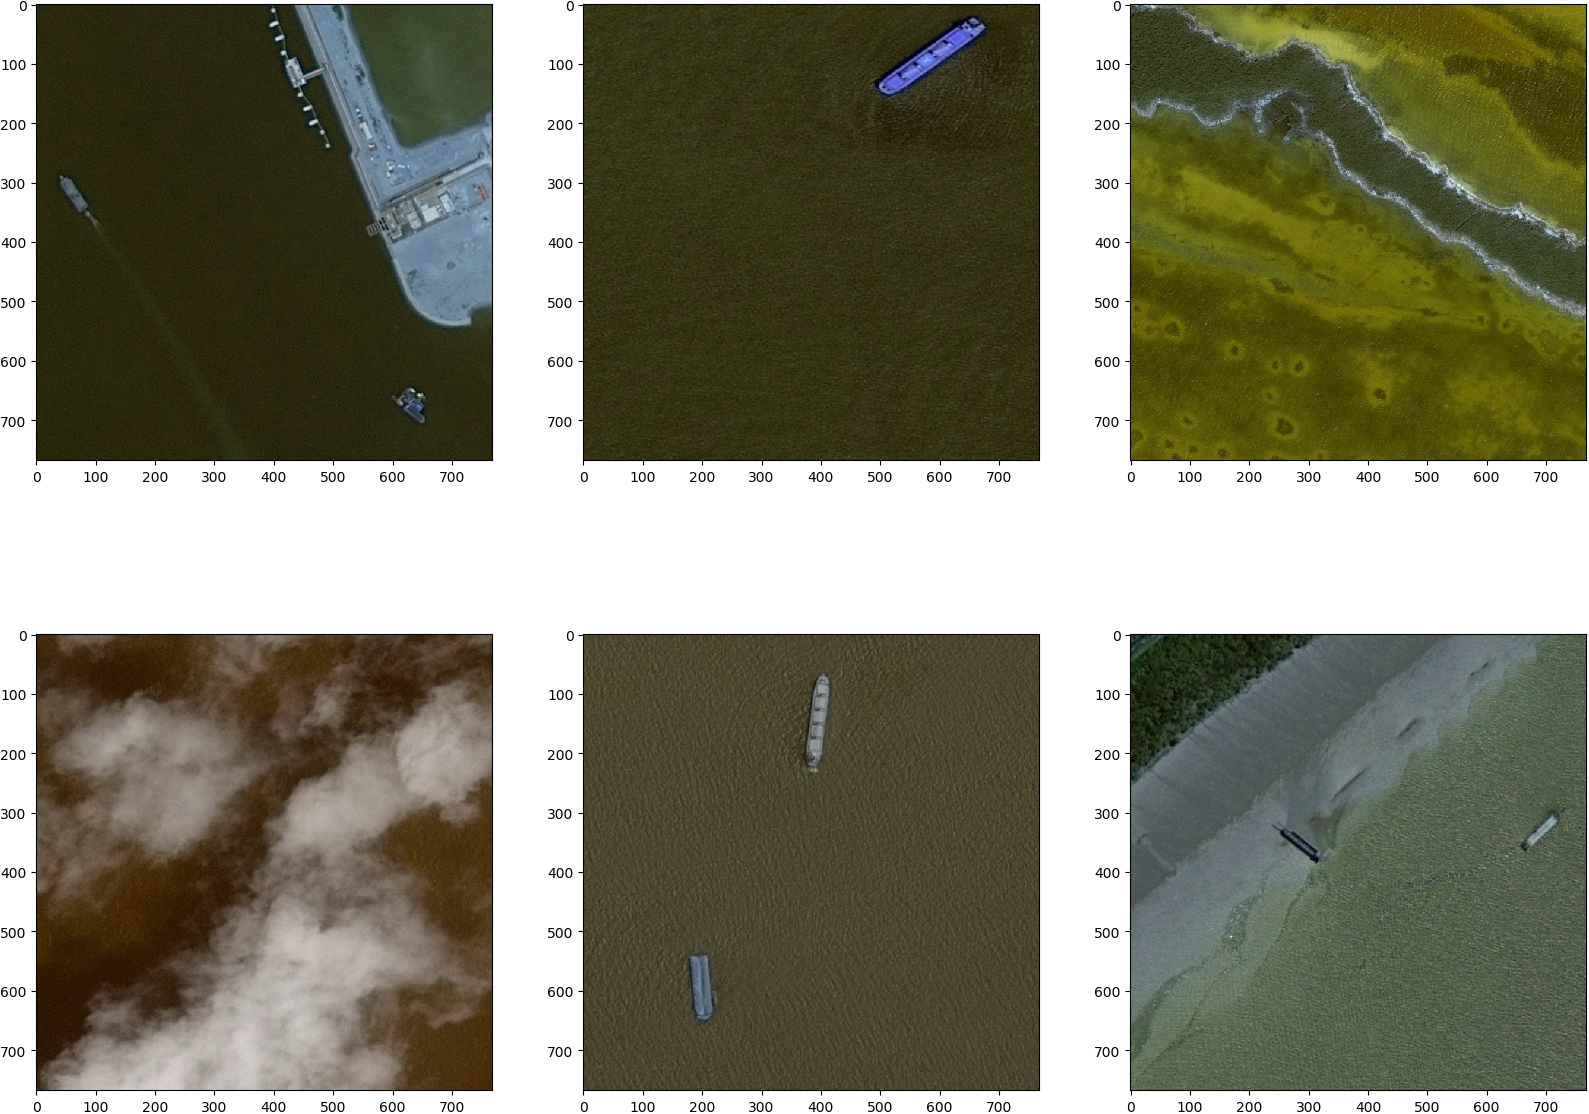
\includegraphics[width=\textwidth]{Pictures/003TrainingSetExamples.png}
	\caption{Training set examples}
	\label{TrainSetExample}
	%\textbf{Figure 2. Hill Climbing algorithm} [15]
\end{figure}

\section{Airbus Ship Dataset}
The Airbus Ship Dataset is an image dataset that was used in the Airbus Ship Detection Challenge \cite{AirbusDataSetChallenge} on \url{www.kaggle.com}. The aim of this competition is to detect ships inside an image taken from an aerial view. As the competition description says, this detection can help multiple organizations such as environmental organization, insurance companies to have knowledge of illegal activities done at sea. A few examples of the training set can be found in Figure \ref{TrainSetExample}.% Todo !!!Challenge with clouds ports etc etc small sizes?


\section{Analysis}
The competition provides both testing and training datasets in a large amount. The train set is composed of \textbf{231723} pictures, of size \textbf{768x768} pixels, in JPEG format, each of them having a set of pixels assigned as being ship pixels. To avoid specifying each pixel separately, for size reasons, the run length encoding is used. Every pixel is numbered from 1 to maximum size, top down, left right order. Pixel (1, 1) will have index 1, pixel (2, 1) index 2 etc. Run length encoding is formed of 2k numbers, the numbers in odd position (1 - indexed) specifies the starting index of a pixel ship sequence, and the ones in even position specifies the length of the sequence.
For example, the sequence: \textit{5 3 10 2}, encodes the ship pixels \textit{\{5, 6, 7, 10, 11\}}. Those encodings are provided via an \textbf{.csv} file, with two columns, \textbf{ImageId} and \textbf{EncodedPixels}. Also, in this file, every ship is given as a separate entry, so a picture can appear multiple times in this file, but at least once. (See table \ref{traindfhead}). The figure \ref{OrigMask} shows the example images with their training masks.\\

\begin{table}[H]
	\centering
	\begin{tabular}{|c|c|l|}
		\hline
		ImageId & EncodedPixels \\ \hline
		00003e153.jpg & NaN         \\ \hline
		0001124c7.jpg & NaN         \\ \hline
		000155de5.jpg & 264661 17 265429 33 266197 33 266965 33 267733...         \\ \hline
		000194a2d.jpg & 360486 1 361252 4 362019 5 362785 8 363552 10 ...   \\ \hline
		000194a2d.jpg & 51834 9 52602 9 53370 9 54138 9 54906 9 55674 ...   \\ \hline
		000194a2d.jpg & 198320 10 199088 10 199856 10 200624 10 201392...  \\ \hline
		000194a2d.jpg & 55683 1 56451 1 57219 1 57987 1 58755 1 59523 ...  \\ \hline
		000194a2d.jpg & 254389 9 255157 17 255925 17 256693 17 257461 ...  \\ \hline
		0001b1832.jpg & NaN  \\ \hline
		00021ddc3.jpg & 108287 1 109054 3 109821 4 110588 5 111356 5 1...  \\ \hline
	\end{tabular}
	\captionof{table}{Train data set sample}\label{traindfhead}
\end{table}

The test set provided by the competition contains \textbf{15607} pictures of the same size as the ones in the training set, and the result that is submitted must also use the run length encoding described above.
\begin{figure}
	\centering
	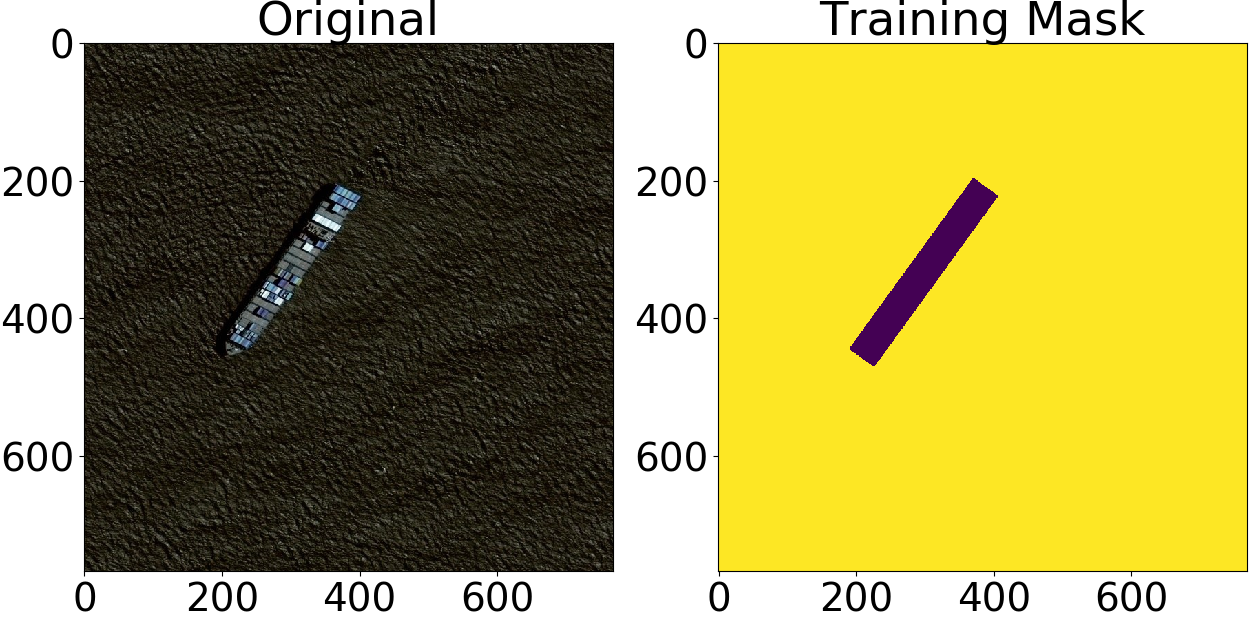
\includegraphics[width=0.75\textwidth]{Pictures/015OrigMaskExample1.png} \\
	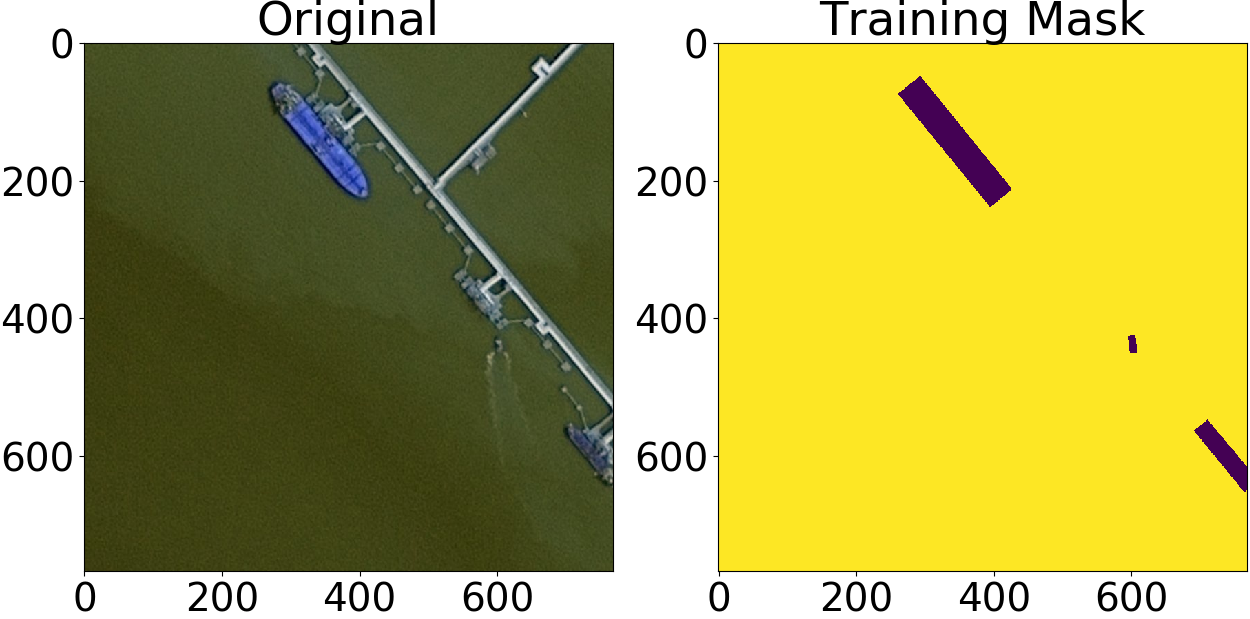
\includegraphics[width=0.75\textwidth]{Pictures/015OrigMaskExample2.png} \\
	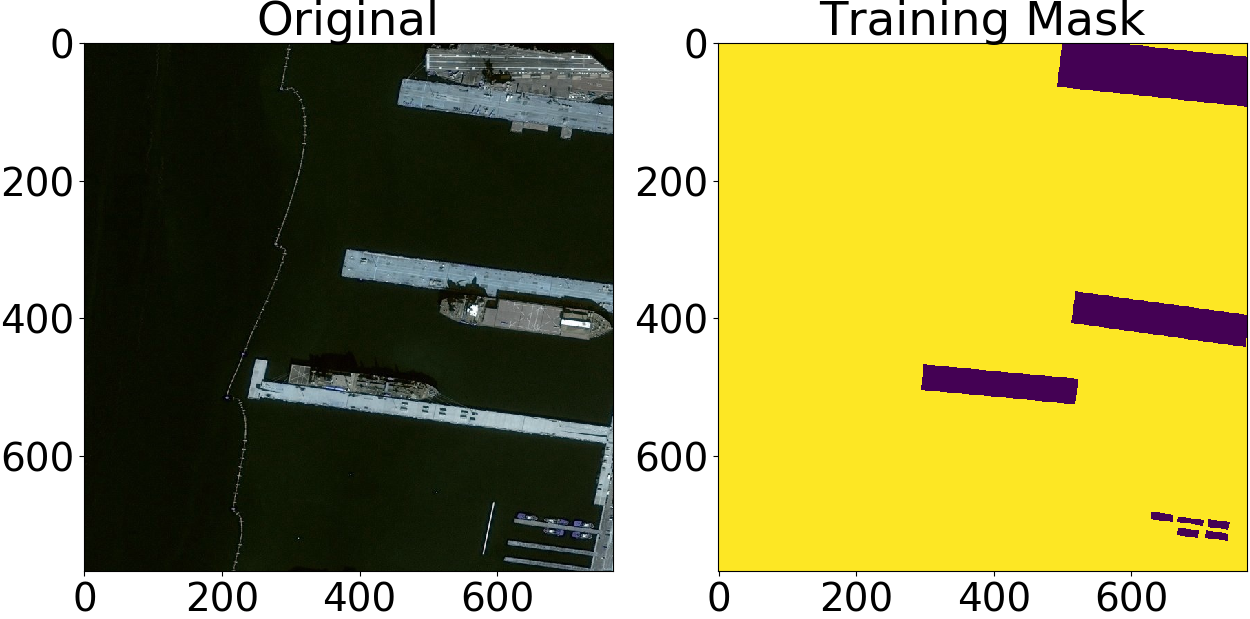
\includegraphics[width=0.75\textwidth]{Pictures/015OrigMaskExample3.png} 
	\caption{Original Images with Training Mask}
	\label{OrigMask}
\end{figure}

On a first inspection of this dataset, it can be observed that there are more pictures with no ship in them (0 encoded pixels), then the number of pictures with ships (as shown in table \ref{shipnoshiptable}). It can be seen that for every picture that have at least one ship in it, there are two pictures with no ship in it.

\begin{table}[H]
	\centering
	\begin{tabular}{|c|c|c|l|}
		\hline
		Total & No Ship Pictures & Ship Pictures \\ \hline
		231723 & 150000 & 81723 \\ \hline
	\end{tabular}
	\captionof{table}{Ship/no ship count training data}\label{shipnoshiptable}
\end{table}

Figure \ref{ShipNumberImage} has a histogram of number of images grouped by number of ships inside an image. The number of pictures that have only 1 ship stands out as being around 35\% from the total number of images with ship, and there are also pictures that contains up to 15 ships.

\begin{figure}
	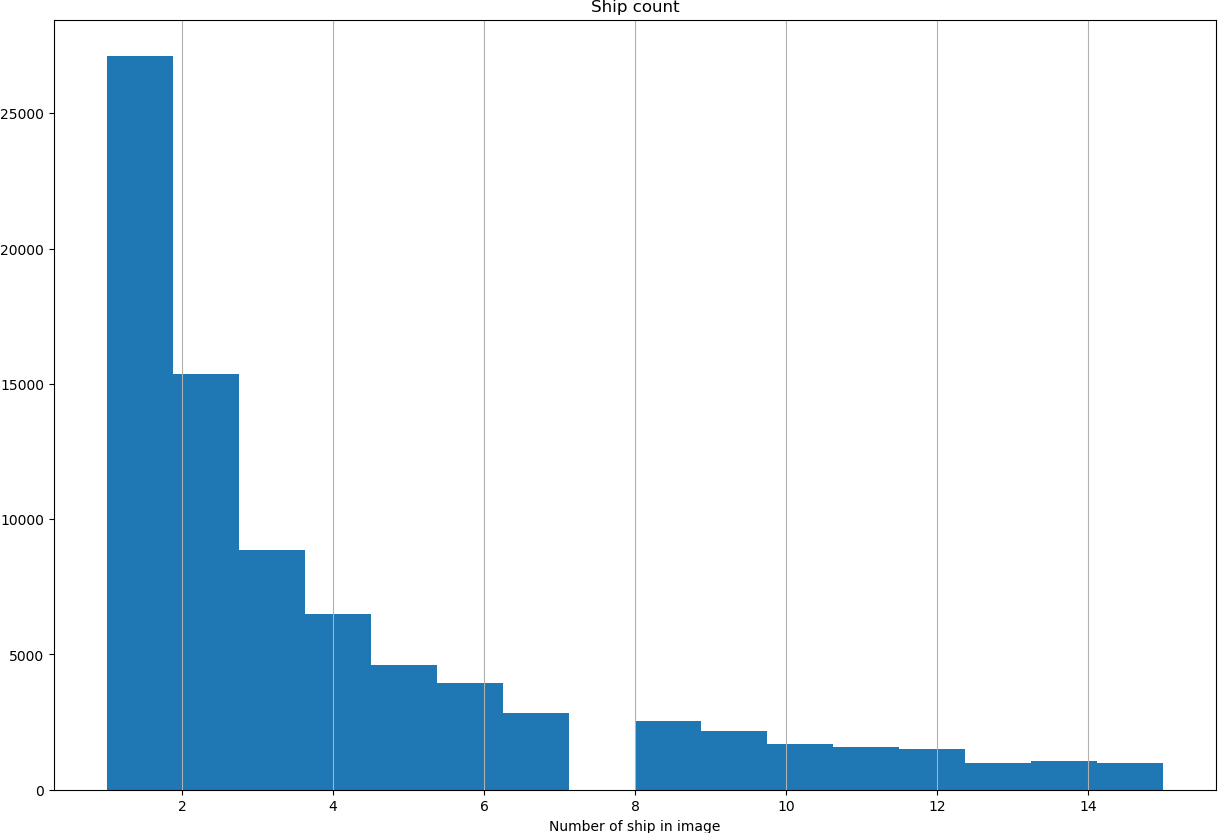
\includegraphics[width=\textwidth]{Pictures/001ShipNumberImage.png}
	\caption{ Number of ships/image}
	\label{ShipNumberImage}
	%\textbf{Figure 2. Hill Climbing algorithm} [15]
\end{figure}

The last metric that should be analyzed in this dataset is the ship size in pixels, to measure the magnitude of the task. As the table \ref{shipzisepixeltable} presents, the average size is around 1500 pixels, with half of the ships in the training set being under 408 pixels in size. Based on this, we can draw the conclusion that one ship that should be detected in the test set forms less than 0.0006\% of the entire image.

\begin{table}
	\centering
	\begin{tabular}{|c|c|c|c|c|c|l|}
		\hline
		Average & Min & Q1 & Median & Q3 & Max\\ \hline
		1,567.40 & 2.00	& 111 & 408.00 & 1550 & 25,904.00 \\ \hline
	\end{tabular}
	\captionof{table}{Ship size in pixels}\label{shipzisepixeltable}
\end{table}

\section{Evaluation Metric}
To evaluate possible solutions for this competition, the $F_2$ score was used. This is defined as follows:
\begin{itemize}
	\item We define a set of thresholds $T = \{0.5, 0.55, 0.6, \dots 0.95\}$.
	\item For every threshold $t \in T$:
	\item the $IoU$ between predicted pixels (pp) and true pixels (tp) of a ship is computed as $IoU = \frac{pp \cap pt}{pp \cup pt}$
	\item if this value is higher than $t$, then this item is consider a true positive (a hit)
	\item if this value is lower than $t$, then this is consider either a false negative (a predicted ship that has no true ship) or a false positive (there is no predicted ship for a true ship)
	\item the $F_2(t) =\frac{5TP(t)}{5TP(t) +4FN(t) + FP(t)}$ is computed
	\item the final score for an image is computed as $FS(image) = \frac{\sum_{t \in T} F_2(t)}{\big{|}T\big{|}}$
\end{itemize}

It is worth mentioning that this metric, in this form, penalizes more false negatives than false positives which means that it encourages rather not to predict a ship if the algorithm is not certain of the ship presence. This will have later implications in this paper. For this reason, the "no-machine algorithm" behaves really well, since this will give a percentage of images with no ships over a dataset. % Data sets

\chapter{Theoretical background}
\lhead{Theoretical background}
\rhead{Radu-George Rusu}
\label{TheoreticalBackground}

This chapter will briefly describe the theoretical models used in the experiments presented in this paper.

\section{Expectation-Maximization}
The Expectation-Maximization (EM) is an algorithmic template for finding the Maximum Likelihood Estimation (MLE) parameters in statistical models which are based on missing or latent data.\\
The Maximum Likelihood Estimation problem can be defined as follows:

\fbox{
\begin{minipage}{\textwidth}
\textbf{MLE Problem}\\
\textbf{Input}\\
Y - set of observed data\\
$p$ - probability distribution that we assume generated the Y data set

\textbf{Output}\\
 $h^{MLE} = \underset{h}{argmax}$  $L(Y | h) = \underset{h}{argmax}$  $p(Y | h) $, where $h$ is the set of distribution parameters
\end{minipage}
}

 When the entire set Y is formed out of observable data, the above problem can be easily solved. A common approach for this instance of the problem, is to take the derivative of the log-likelihood function and solve it for $h$. However, real life data is not always fully observed, and inside of the given data we have latent variables. In this particular case, the above-mentioned method doesn't work anymore, and an EM approach can be used.
 
 In the case of latent data we can consider the Y set as being a reunion between $X \cup Z = Y$, where X is the set of visible data, and Z is the set of hidden/latent data. The initial method doesn't work since it is impossible to compute $p(Z | h)$.
 
 \begin{figure}[H]
 	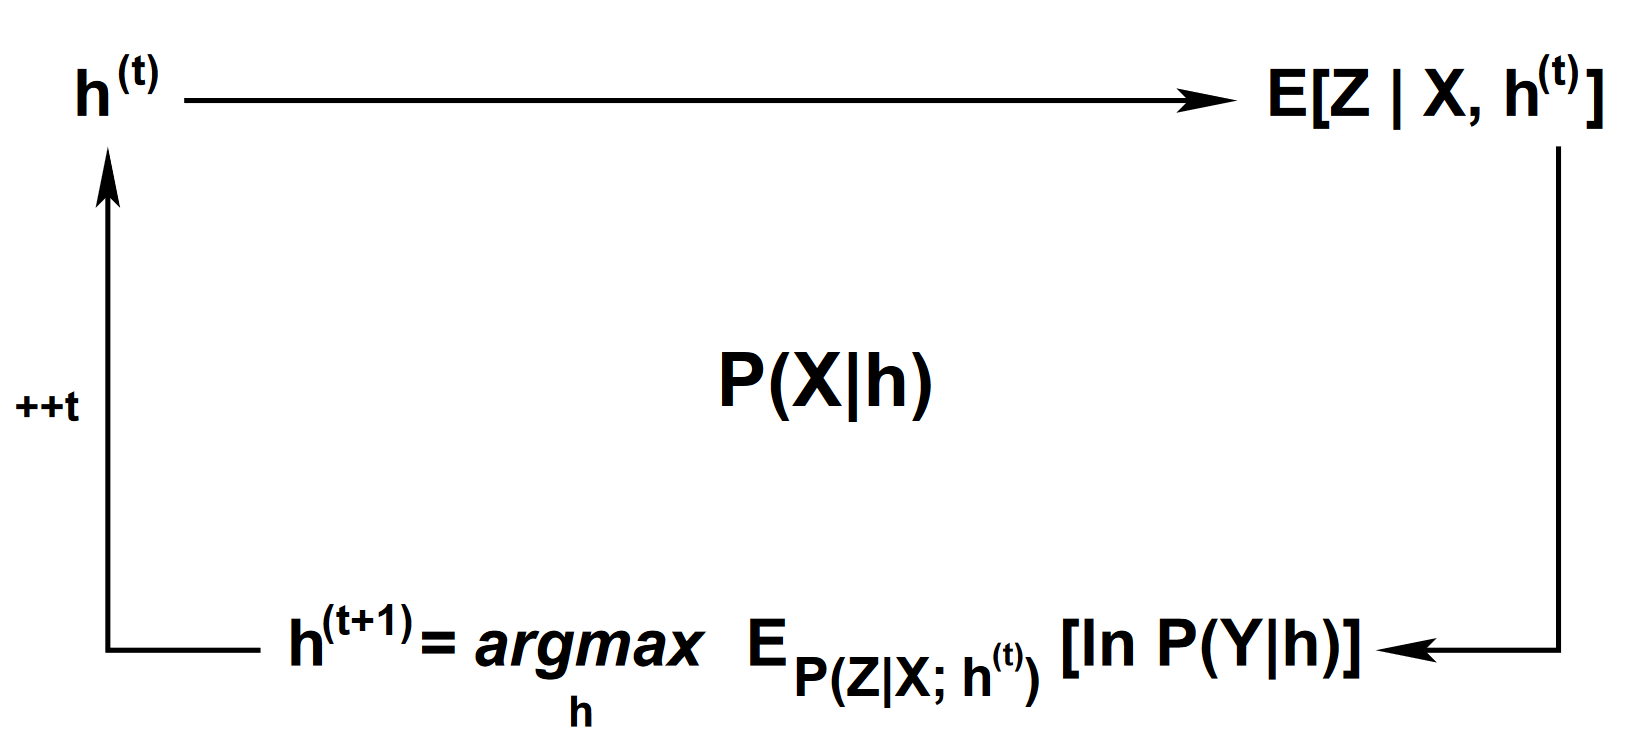
\includegraphics[width=\textwidth]{Pictures/004EMScheme.png}
 	\caption{EM Algorithm \cite{emCiortuz}}
 	\label{EmScheme}
 	%\textbf{Figure 2. Hill Climbing algorithm} [15]
 \end{figure}
 
 The EM algorithm (as show in \ref{EmScheme}) applies an iterative method, that for each iteration computes two steps:
 \begin{itemize}
 	\item E-Step: expectation of the latent variables, based on the distribution parameters from the previous iteration and the visible data ($\mathbf{E[Z | X, h^{(t)}]}$).
 	\item M-Step: based on the results from the E-Step, the latent variables, can be considered as observed and the $h$ parameters for this step can be solved like in the classic MLE problem.
 \end{itemize}

In the most basic form of this algorithm, the initial values for $h^{(0)}$ are randomly selected, and as a stop condition a maximum number of iterations is  used, but these two conditions can vary from problem to problem.
 
 
\section{Neural Networks for object detection}
In computer vision and object detection/recognition in images, the classical neural networks involves a high number of weights that have to be learned, which in turn, makes the networks work slow on images that are bigger in size and sometimes even impractical. The main advantage of the \textbf{Convolutional Neural Networks (CNN)} \cite{ConvNeuralNetwork} is the idea of using the convolution operator (\ref{Convolution}), which drastically reduces the number of weights to be learned during training phase and makes them usable in practice.

 \begin{figure}[H]
	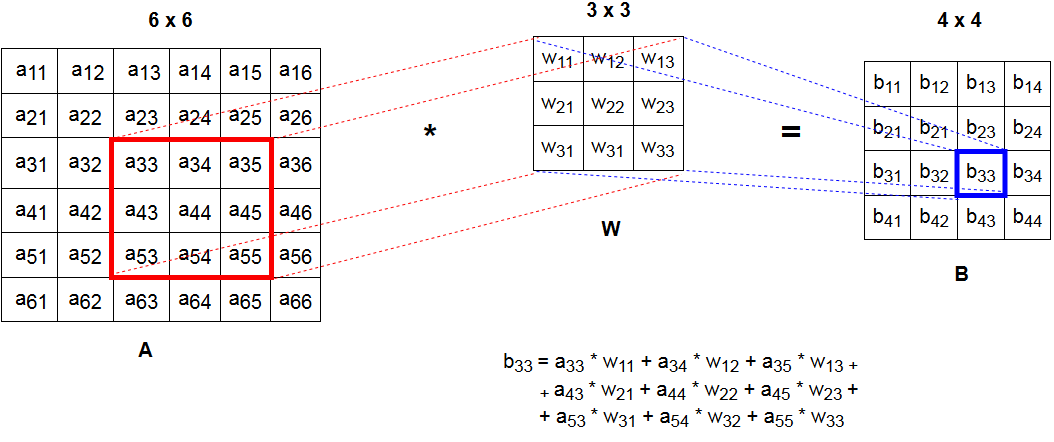
\includegraphics[width=\textwidth]{Pictures/006Convolution.png}
	\caption{Convolution operator \cite{ConvNeuralNetwork}}
	\label{Convolution}
	%\textbf{Figure 2. Hill Climbing algorithm} [15]
\end{figure}

Other two popular operators are the AveragePooling and MaxPooling, which as the name suggests, just extract either the average or the maximum value of the values in the corresponding square. Although these operators doesn't have as much expression power as the linear combination \ref{Convolution}, they don't have any weights to be learned during the training phase.

The convolution operator result size depends on the following variables:
\begin{itemize}
	\item $n$ - size of the input image (considering the input image is squared)
	\item $f$ - size of the filter (also squared)
	\item $p$ - padding of the initial image
	\item $s$ - stride of the convolution operation
\end{itemize}
The convolution operator result size is:
$$ (n, n) * (f, f) = \bigg( \bigg\lfloor \frac{n + 2 \times p - f}{s} + 1 \bigg\rfloor , \bigg\lfloor \frac{n + 2 \times p - f}{s} + 1 \bigg\rfloor \bigg)$$

To observe the advantages of CNN over the classical NN we can take an example of a network formed only of two layers. A first one of size $1024\times1024$ which can be viewed as the input image, that is given in grayscale, and a second layer of size $512\times512$, which is a first feature extraction layer.

In a classical neural network every input from the first layer must be connected with every output on the second layer, and every connection has it's own weight, which, in the above case, would result in computing $1024 \times 1024 \times 512 \times 512 = 274,877,906,944$ weights. Also, in computer vision problem there is a need of more than one intermediate layer to extract the features inside an image.

In the case of CNNs, the only weights that have to be computed for a layer are the values inside the kernel, which in the above example can be considered a kernel of size $512 \times 512 = 262,144‬$ with a stride of 1 and no padding. The number of weights that will be learned it's way less than in the case of classical neural networks, which allows more layers, and makes the CNN more practical for this problem. Also, in practical cases, the convolution operator can be an average/maximum over the target values, instead of a linear combination, and there will be no weights to learn on that level.

 \begin{figure}[H]
	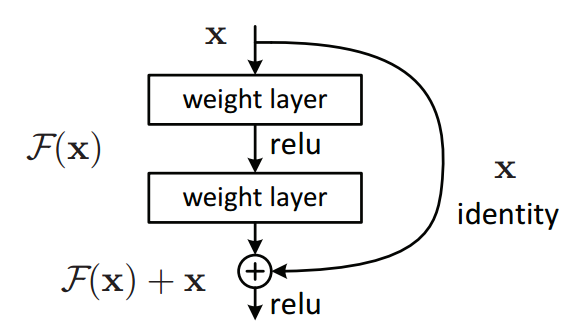
\includegraphics[width=\textwidth]{Pictures/007SkipConnection.png}
	\caption{Residual Block \cite{ResNetPaper}}
	\label{SkipConnection}
	%\textbf{Figure 2. Hill Climbing algorithm} [15]
\end{figure}

Another issue that occurs in practical object detection in image cases, is the depth of the network. In order to learn complex features inside an image, a neural network needs a high number of layers, to have space for learning every feature, which, in practice, leads to the vanishing gradient problem \cite{ResNetPaper}. This problem makes the training of these networks hard or even impossible, depending on the task. To solve this \textbf{Residual Networks} \cite{ResNetPaper} were developed.

The fundamental idea of these networks is the addition of the residual blocks (\ref{SkipConnection}). In this blocks, the inputs are once again added to the output value of a later layer, before the activation function, avoiding a "squishing" derivative, which in turn will result in a higher overall derivative of the entire block.

With these methods, neural networks structures with 34, 50 or 152 layers were developed and used as show in \ref{ResNetExample}.

 \begin{figure}[H]
	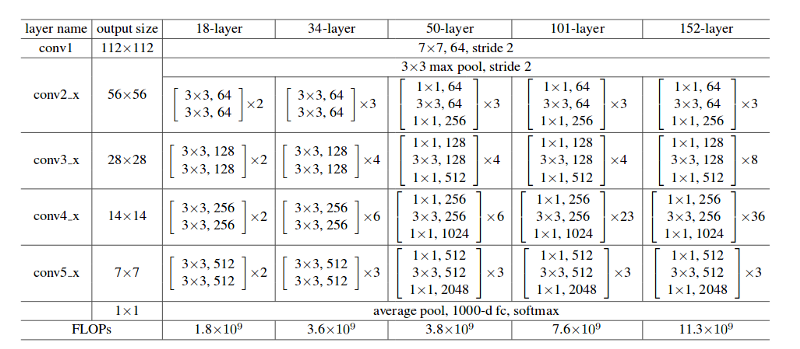
\includegraphics[width=\textwidth]{Pictures/008ResNetExample.png}
	\caption{Residual Networks Structure \cite{ResNetPaper}}
	\label{ResNetExample}
	%\textbf{Figure 2. Hill Climbing algorithm} [15]
\end{figure}

The neural networks described above behave well on object recognition and object detection problems. Another common case in image processing is the segmentation problem, where similar pixels inside a picture must be grouped together. In this particular case, the CNN might not work well in the form described above, because every pixel of the image can have it's own classification, and the convolution operator is specialized in contracting image features, hence reducing the number of outputs of the network. To solve this problem, \textbf{U-Nets} networks \cite{Unet} have been developed. The name U-Net comes from the visual representation of the architecture (\ref{UnetArchitecture}) which resembles the U letter. There are two parts of this architecture, the contracting path, and the expansive path. The contracting path behaves as an usual convolutional neural network extracting features from the image. The expansive path uses the Transposed Convolution Operator \cite{ConvolutionOperatorPaper}, which helps the networks reconstruct the image at the initial resolution, from the feature vector that was computed by the contracting path. 

 \begin{figure}[H]
	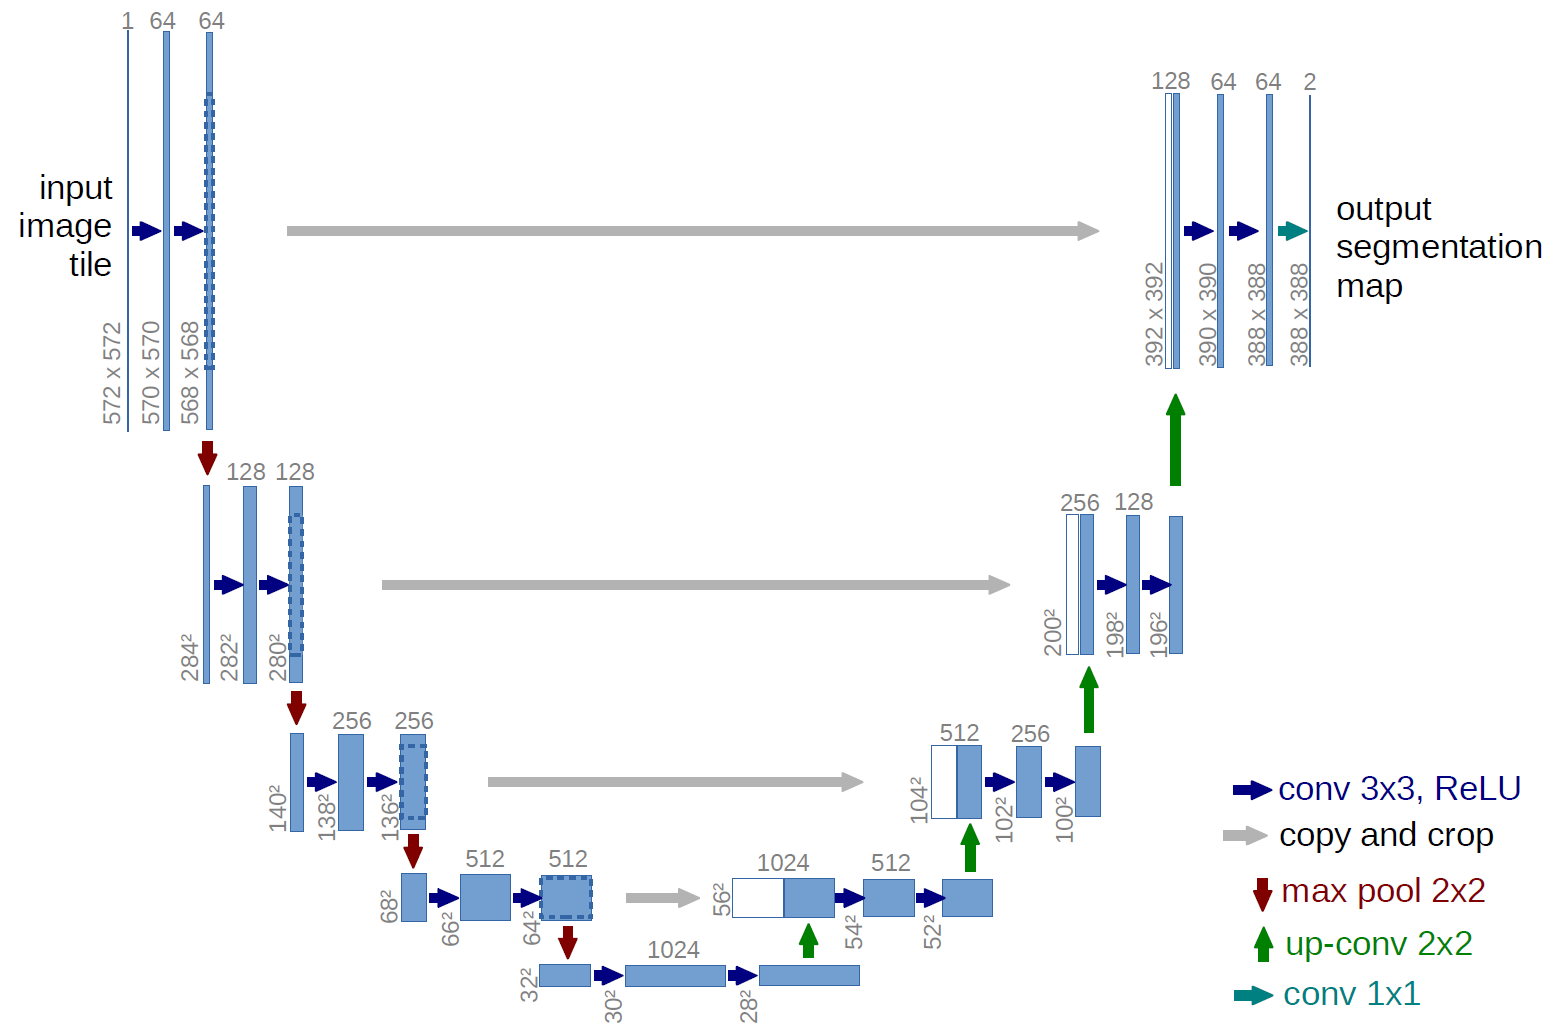
\includegraphics[width=\textwidth]{Pictures/012Unet.png}
	\caption{U-Net Architecture \cite{Unet}}
	\label{UnetArchitecture}
	%\textbf{Figure 2. Hill Climbing algorithm} [15]
\end{figure} % Algorithms

\chapter{Experiment setup}
\lhead{Experiment setup}
\rhead{Radu-George Rusu}
\label{ExperimentSetup}

This chapter will present the thought process and the setup that was used to run the experiments on the dataset presented in Chapter \ref{DatasetChapter}.

\section{Initial idea}

Taking a high level look through the training data set, a general case can be seen: pictures are taken at sea (no port in site) and as such, they are also conceived from water and ships (which can divide pixels in two group as shown in image \ref{ShipExampleAtSea}). If the images are moved into grayscale, and their histogram is computed (\ref{ImageHistogram}), then the pixels of the image can be split into two groups, both generated by a Gaussian distribution, which will also give the ship/no-ship classification. This problem is a classical problem that can be solved using EM algorithm.

\begin{figure}[h]
	\centering
	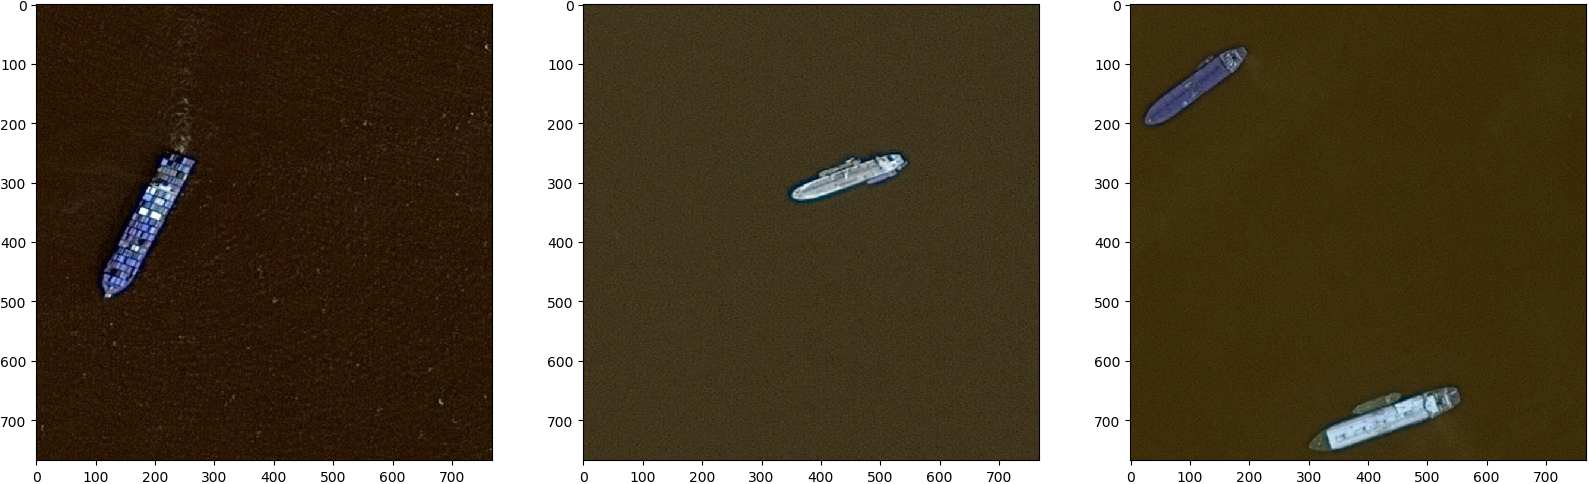
\includegraphics[height=0.2\textheight]{Pictures/002ShipExampleatSea.png}
	\caption{Ships at sea}
	\label{ShipExampleAtSea}
\end{figure}

\begin{figure}[h]
	\centering
	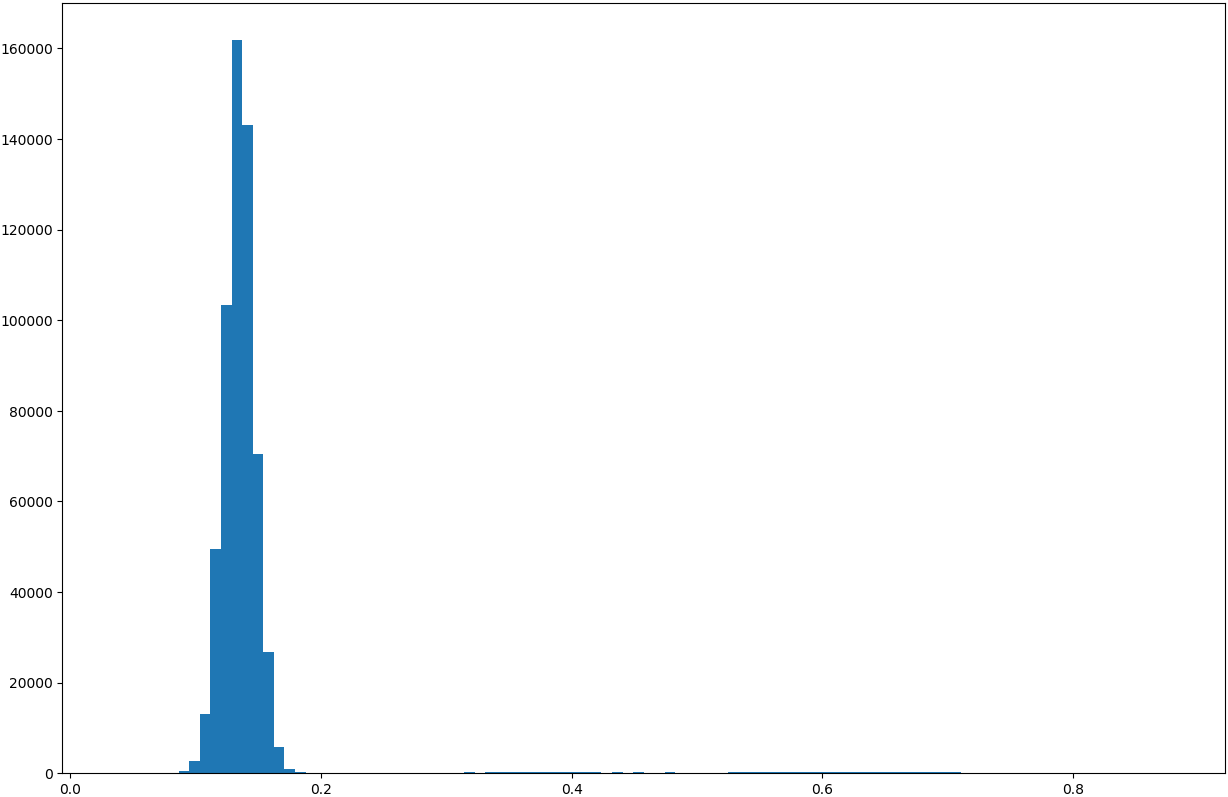
\includegraphics[width=\textwidth]{Pictures/005ImageHistogram.png}
	\caption{Histogram of grayscale at sea image}
	\label{ImageHistogram}
\end{figure}

\section{Expectation-Maximization}
For the rest of this section the following notations will be used:
\begin{table}[H]
	\centering
	\begin{tabular}{cp{0.8\textwidth}}
		$\mathbf{p(x_i)}$ & probability of the pixel $i$ \\ 
		$\mathbf{\mathcal{N} (x_i | \mu_s , \sigma_s)}$ & PDF value of pixel $i$ generated by the ship Gaussian distribution \\
		$\mathbf{\mathcal{N} (x_i | \mu_b , \sigma_b)}$ & PDF value of pixel $i$ generated by the background Gaussian distribution \\
		$\mathbf{G_s}$ & random variable that represents the presence of ships in the image\\
		$\mathbf{G_b}$ & random variable that represents the presence of background in the image\\
		$\mathbf{n}$ & number of pixels in the image 
	\end{tabular}
	\caption{Notations}\label{notations}
\end{table}
In order to apply EM to our problem, some adaptations must be done. First, we will be considering two random variables $G_s$ and $G_b$, both in $[0, 1]$, which will represent the presence of ship, respectively background in the image. The hidden variables in this problem will be some random variables that assign every pixel either to the ship group or background group. Also, considering the observation from the beginning of this section, the value of every pixel will be a probability generated by the two Gaussians as follows:
$$ p(x_i) = \mathcal{N}(x_i | \mu_s, \sigma_s) P(G_s) + \mathcal{N}(x_i | \mu_b, \sigma_b) P(G_b) $$

\subsection{E-Step}

The likelihood of the data will be computed as follows:

$$L = \prod_{i=1}^{n} p(x_i) = \prod_{i=1}^{n} \mathcal{N}(x_i | \mu_s, \sigma_s) P(G_s) + \mathcal{N}(x_i | \mu_b, \sigma_b) P(G_b)$$

Next we compute the mean of the likelihood for this iteration:
$$Q(h | h^{(t)}) = E_{P(G | x, h^{(t)})}\bigg[\prod_{i=1}^{n} \mathcal{N}(x_i | \mu_s, \sigma_s) P(G_s) + \mathcal{N}(x_i | \mu_b, \sigma_b) P(G_b)\bigg]$$
$$=\prod_{i=1}^{n} E_{P(G | x, h^{(t)})}\bigg[\mathcal{N}(x_i | \mu_s, \sigma_s) P(G_s) + \mathcal{N}(x_i | \mu_b, \sigma_b) P(G_b)\bigg] $$
$$=\prod_{i=1}^{n}E_{P(G | x, h^{(t)})}\bigg[\mathcal{N}(x_i | \mu_s, \sigma_s) P(G_s)\bigg] + E_{P(G | x, h^{(t)})}\bigg[\mathcal{N}(x_i | \mu_b, \sigma_b) P(G_b)\bigg] $$
$$=\prod_{i=1}^{n} \mathcal{N}(x_i | \mu_s, \sigma_s) E_{P(G | x, h^{(t)})} P(G_s) + \mathcal{N}(x_i | \mu_b, \sigma_b) E_{P(G | x, h^{(t)})} P(G_b) $$

Now the estimation for the $P(G_s)$ and $P(G_b)$ must be computed considering that:
$$P(G_s) = \frac{1}{n} \sum_{t = 1}^{n}P(G_s | x_i)$$
$$P(G_b) = \frac{1}{n} \sum_{t = 1}^{n}P(G_b | x_i)$$
which leads to:
$$E_{P(G | x, h^{(t)})} P(G_s) = \sum_{i=1}^{n} E_{P(G | x, h^{(t)})} P(G_s | x_i) $$
$$E_{P(G | x, h^{(t)})} P(G_b) = \sum_{i=1}^{n} E_{P(G | x, h^{(t)})} P(G_b | x_i) $$

The ML estimation of the above elements is as follows \cite{EMObjectConcealement}:
$$E_{P(G | x, h^{(t)})} P(G_s | x_i) = \frac{\mathcal{N}(x_i | \mu_s^{(t)}, \sigma_s^{(t)}) P(G_s)^{(t)}}{\mathcal{N}(x_i | \mu_s^{(t)}, \sigma_s^{(t)}) P(G_s)^{(t)} + \mathcal{N}(x_i | \mu_b^{(t)}, \sigma_b^{(t)}) P(G_b)^{(t)}}	$$

$$E_{P(G | x, h^{(t)})} P(G_b | x_i) = \frac{\mathcal{N}(x_i | \mu_b^{(t)}, \sigma_b^{(t)}) P(G_b)^{(t)}}{\mathcal{N}(x_i | \mu_s^{(t)}, \sigma_s^{(t)}) P(G_s)^{(t)} + \mathcal{N}(x_i | \mu_b^{(t)}, \sigma_b^{(t)}) P(G_b)^{(t)}}	$$

\subsection{M-Step}
At this point, considering the previous section, we have a form for the expectation of the likelihood function, so the Maximization step can be applied. By taken the above formulas and computing the derivatives based on the parameters we obtain the following actualization rules \cite{EMObjectConcealement}: \\

\begin{table}[H]
	\centering
	\begin{tabular}{cc}
		\begin{minipage}{0.5\textwidth}
			$$\mu_s^{(t+1)} = \frac{\sum_{i=1}^{n}P(G_s | x_i) * x_i}{\sum_{i=1}^{n}  P(G_s | x_i)}$$
		\end{minipage} &
		\begin{minipage}{0.5\textwidth}
			$$\mu_b^{(t+1)} = \frac{\sum_{i=1}^{n}P(G_b | x_i) * x_i}{\sum_{i=1}^{n} P(G_b | x_i)}$$ 
		\end{minipage} \\ 
		\\
		\begin{minipage}{0.5\textwidth}
			$$\sigma_s^{(t+1)} = \frac{\sum_{i=1}^{n} P(G_s | x_i) (x_i - \mu_s^{(t)})^2}{\sum_{i=1}^{n} P(G_s | x_i)}$$
		\end{minipage} &
		\begin{minipage}{0.5\textwidth}
			$$\sigma_b^{(t+1)} = \frac{\sum_{i=1}^{n} P(G_b | x_i) (x_i - \mu_b^{(t)})^2}{\sum_{i=1}^{n} P(G_b | x_i)}$$
		\end{minipage} \\
		\\
		\begin{minipage}{0.5\textwidth}
			$$P(G_s)^{(t+1)} = \frac{1}{n} \sum_{t = 1}^{n}P(G_s | x_i)$$
		\end{minipage} &
		\begin{minipage}{0.5\textwidth}
			$$P(G_b)^{(t+1)} = \frac{1}{n} \sum_{t = 1}^{n}P(G_b | x_i)$$
		\end{minipage} \\
	\end{tabular}
\end{table}

The initialization values for the EM parameters were given as a random value between $0$ and $1$, for $\mu$ and $\sigma$. The $P(G_b)$ had an initial value of $0.9$ and $P(G_s)$ a value of $0.1$, since we expect to have more background than ships in an image. In order to stop the algorithm, a maximum iteration value of 12 was used, without any other restrictions. Parameter learning was executed on a resized ($256\times256$) for performance reasons, and the classification phase was run on the full-size image. After the parameters were computed, the following rule was used to classify pixels as either ship or background:
\begin{itemize}
	\item if $P(G_s | x_t) \geq P(G_b | x_t)$ then classify $x_t$ as \textbf{ship}
	\item if $P(G_s | x_t) < P(G_b | x_t)$ then classify $x_t$ as \textbf{background}
\end{itemize}
Before applying the EM algorithm, all images were converted to grayscale so that every pixel has only one characteristic value and not 3, like in the RGB format. Another preprocessing technique used was a Gaussian filter with the purpose of smoothing the edges in the picture. 


\subsection{EM results}
\label{emres}
After applying the EM algorithm over a subset of images we obtain results as shown in \ref{init_result}.

\begin{figure}[h]
	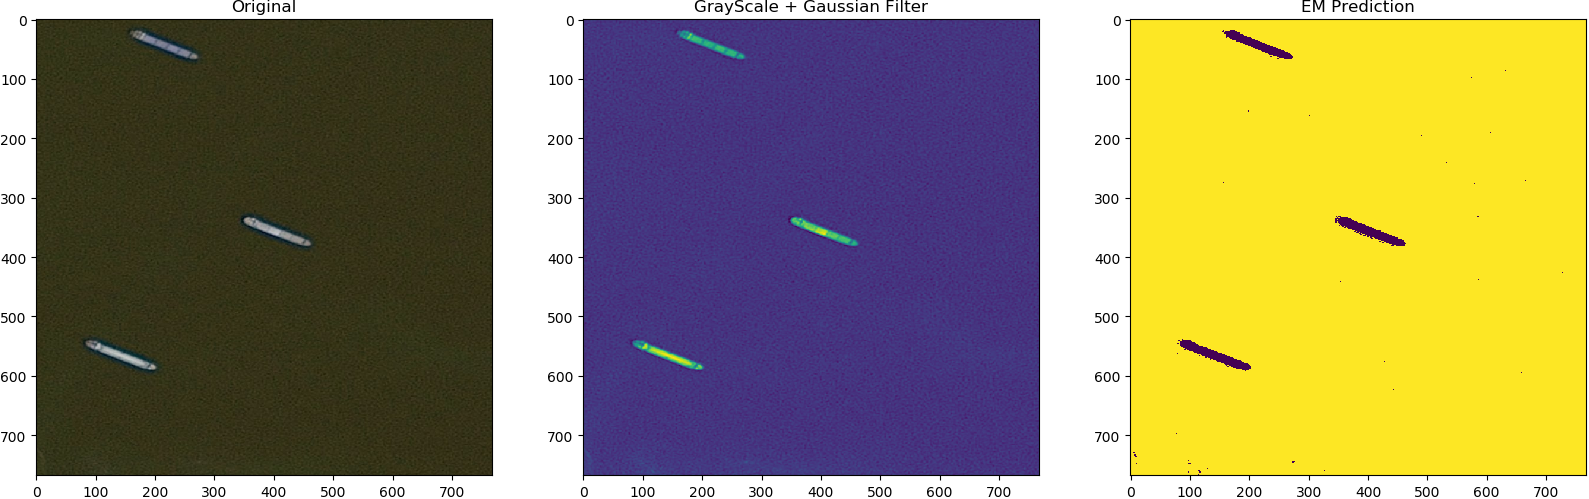
\includegraphics[width=\textwidth]{Pictures/009Ex1.png}\\
	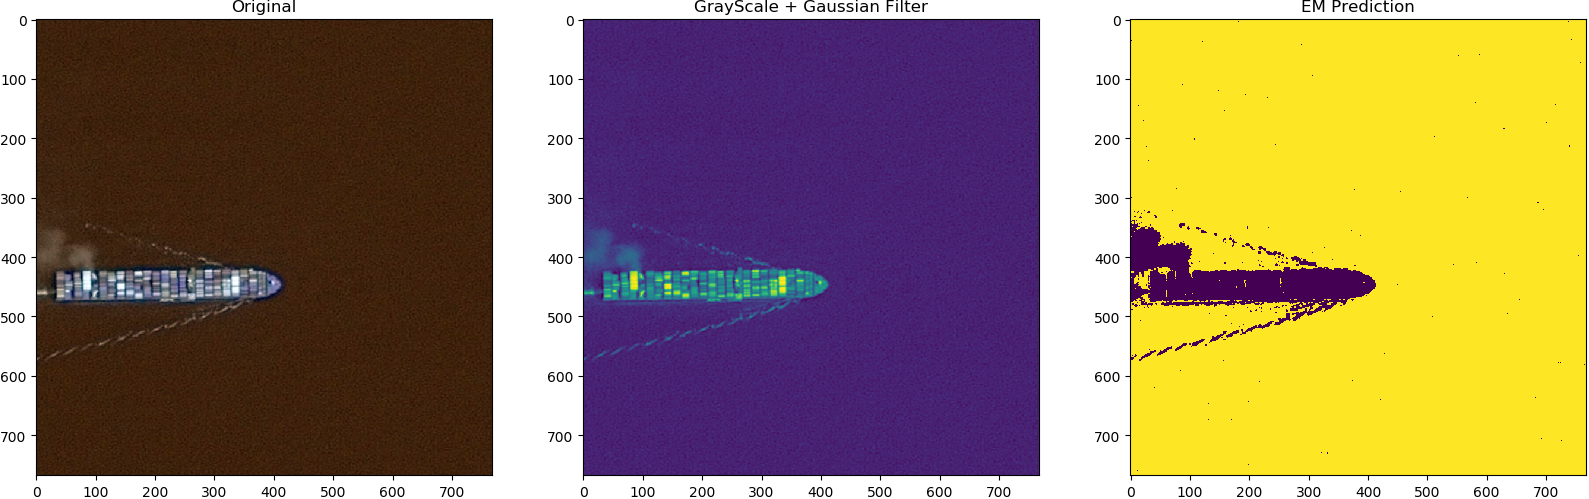
\includegraphics[width=\textwidth]{Pictures/009Ex2.png}\\
	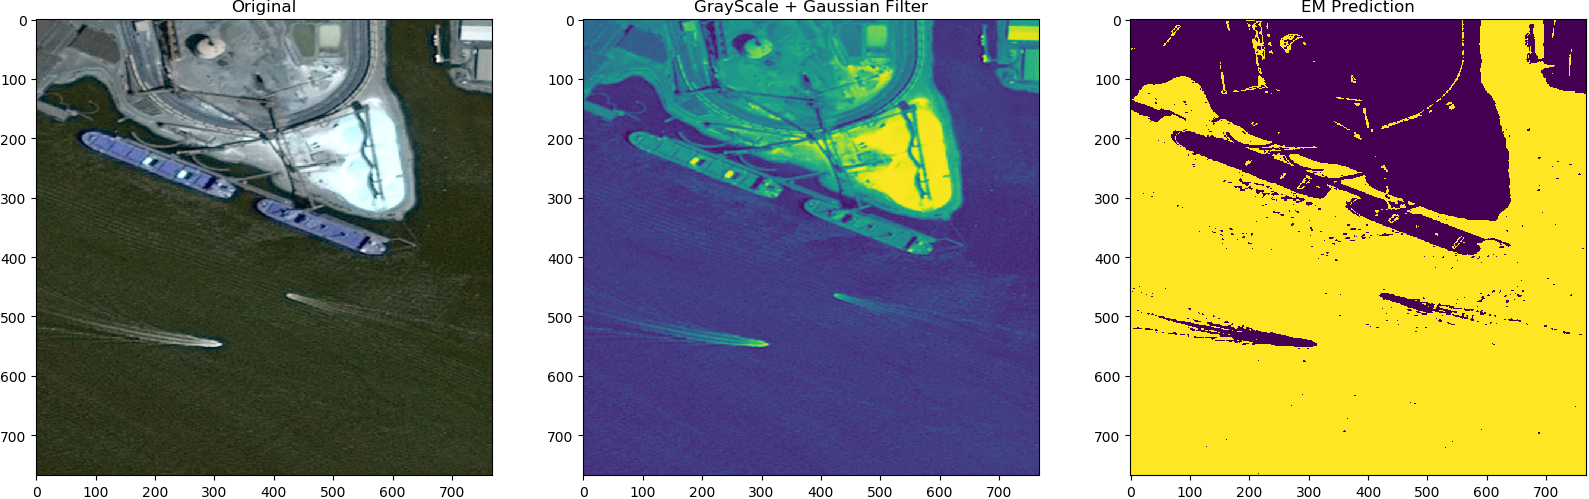
\includegraphics[width=\textwidth]{Pictures/009Ex3.png}
	\caption{Initial Results}
	\label{init_result}
\end{figure}

It can be observed that in "at sea" pictures, the algorithm behaves quite good
(although it still predicts some pockets of pixels that are not ships), but in
the port pictures the algorithm detects the port as being a ship as well.
Also, because the algorithm enforce that every pixel is generated by the
formula specified earlier, in case of no-ship picture this algorithm will still
detect ships.

After this steps, 3 main caveats of the EM algorithm have been identified:
\begin{itemize}
	\item [1.] the algorithm is classifying pixels in images that have no ship (the algorithm is not able to distinguish this particular case) \textbf{(P1)}
	\item [2.] the algorithm is classifying small pockets of pixels as ship (usually waves that visually distinguish themselves from the rest of the water) \textbf{(P2)}
	\item [3.] in the images that have ports, the algorithm identifies the port pixels as being ships (mainly because of the color similarity between them) \textbf{(P3)}
\end{itemize}

\section{Region Proposal Solution}
\label{regPropSol}
Since the EM algorithm by itself had the caveats mentioned in \ref{emres}, a pipeline \ref{arch1} around the algorithm was developed.
To solve \textbf{(P1)} a Residual Network (with a ResNet34 architecture \cite{ResNetPaper}) was used for classifying the images, in images with ships and with no ships. Using this, the EM algorithm could be ran, only on the images that are certain to have ships. The network was train on \textbf{10000} images, plus rotation preprocessing with -90 and 90 degrees, randomly selected from the train set of the initial problem.

\begin{figure}[h]
	\centering
	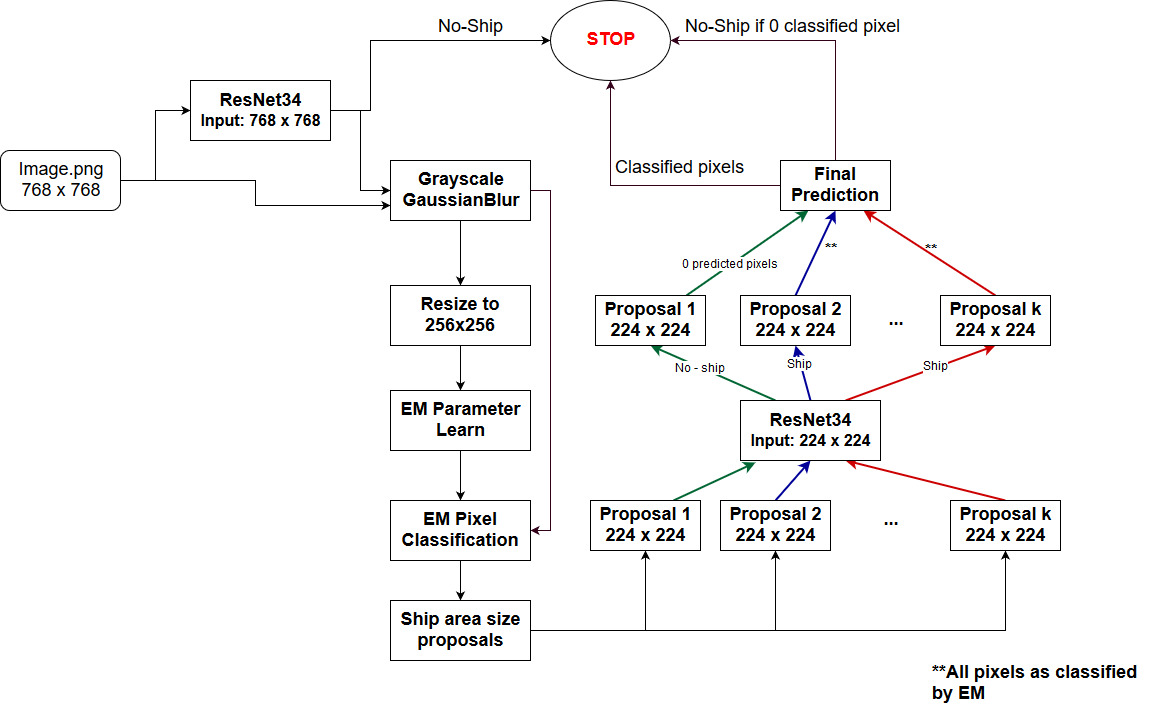
\includegraphics[angle=90,height=0.8\textheight]{Pictures/010Architecture1.jpg}
	\caption{Region Proposal}
	\label{arch1}
\end{figure}

After this phase, on the images classified as ship images, the EM algorithm was ran. In order to solve \textbf{(P2)}, a de-noising technique was applied on the image result. The fast de-noising Nl means from cv2 library was chosen, which helps removing small pockets of isolated pixels, and also smoothen the edges of the ships. The method is applied for each pixel, by taken a surrounding area of the target pixel and averaging it with similar areas in the image.

Finally, in the third phase, another Residual Network was used in order to remove the ship labels from port pixels. This is a more difficult issue to solve, since ports have a color scheme really similar to ships.
\begin{itemize}
	\item First we split the EM predicted image in 25 crops, of size $224 \times 224$.
	\item Only the windows that have at least 35 (\ref{shipzisepixeltable}) pixels predicted as ship will be considered as a possible valid prediction.
	\item This Residual Network also used the ResNet34 architecture \cite{ResNetPaper} that is capable of classifying the idea of ship/no-ship, and was trained on $224\times224$ random crops ($\sim \mathbf{50000}$, taken the same way as the selection for prediction).
\end{itemize}

\section{Region Proposal Example Run}
The following figures shows a picture in different stages of processing:
\begin{enumerate}
	\item \ref{orig_pic} - the input image of the algorithm (left), the image after the Gaussian filter was apply and the encoding was moved to grayscale (right)
	\item \ref{em_pic} - the classification result after the em algorithm where the yellow pixels are background, and the purple one are ships(left), and the em result after the de-noising technique has been applied(right)
	\item \ref{propose_pic} - the 9 propose regions for second classification
	\item \ref{final_result_pic} - the final result compared to the initial picture
\end{enumerate}

\begin{figure}[H]
	\centering
	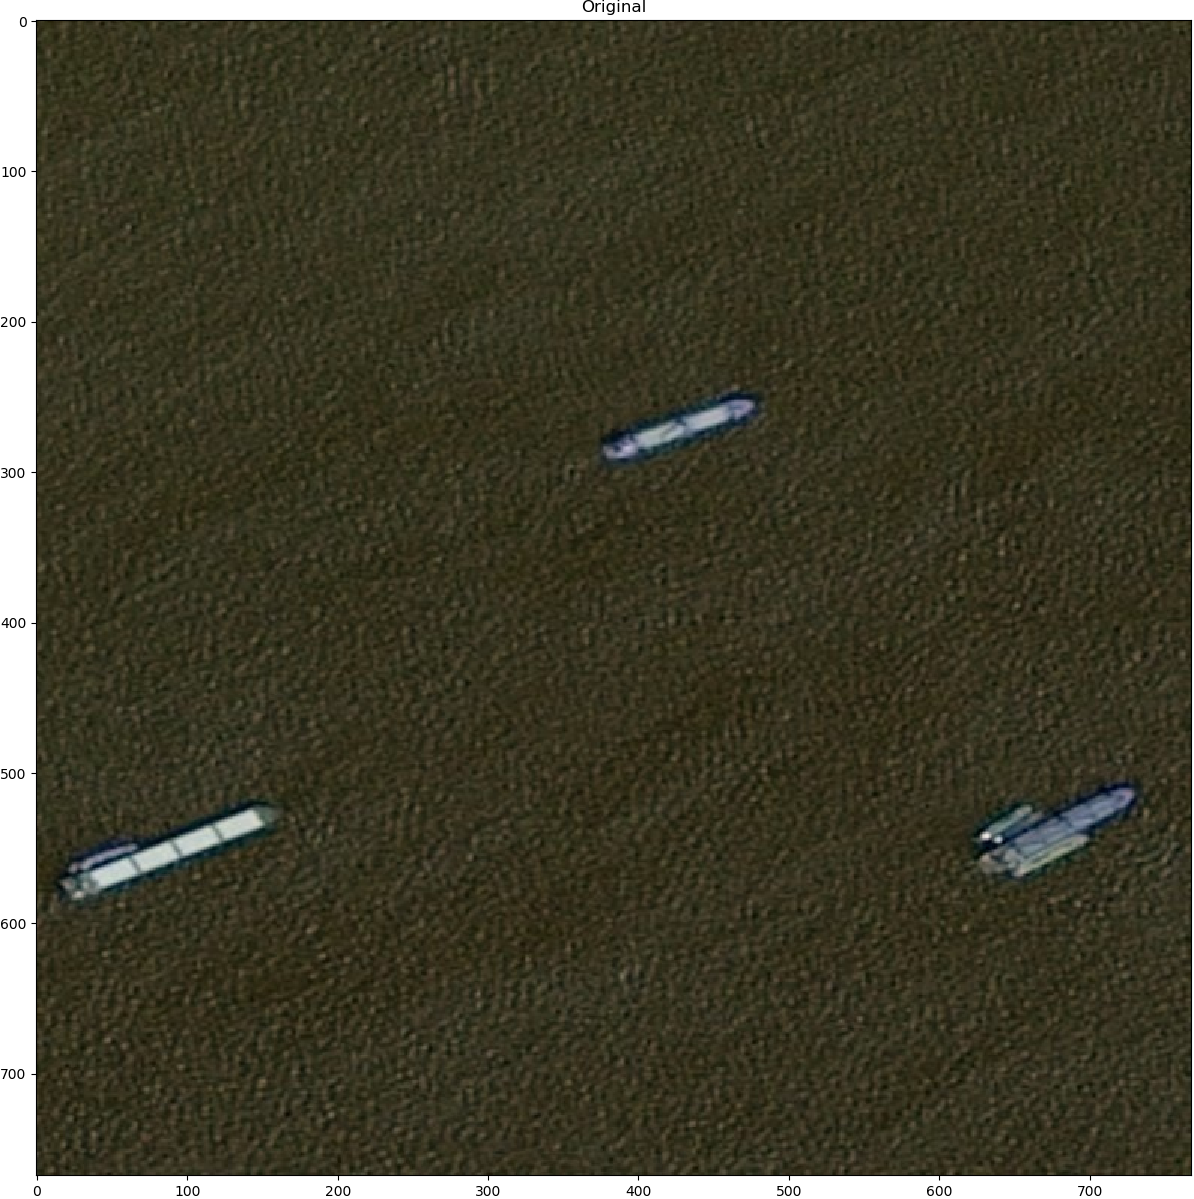
\includegraphics[width=0.45\textwidth]{Pictures/011Original.png}
	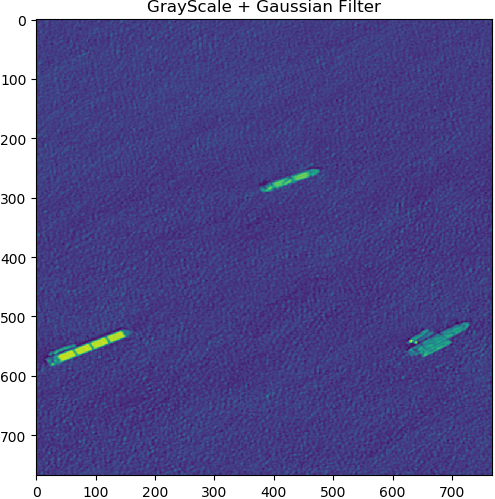
\includegraphics[width=0.45\textwidth]{Pictures/011GrayScale.png}
	\caption{Input/Original Picture, Grayscale and Gaussian Filtering}
	\label{orig_pic}
\end{figure}

\begin{figure}[H] 
	\centering
	\includegraphics[width=0.45\textwidth]{Pictures/011EMPred.png}
	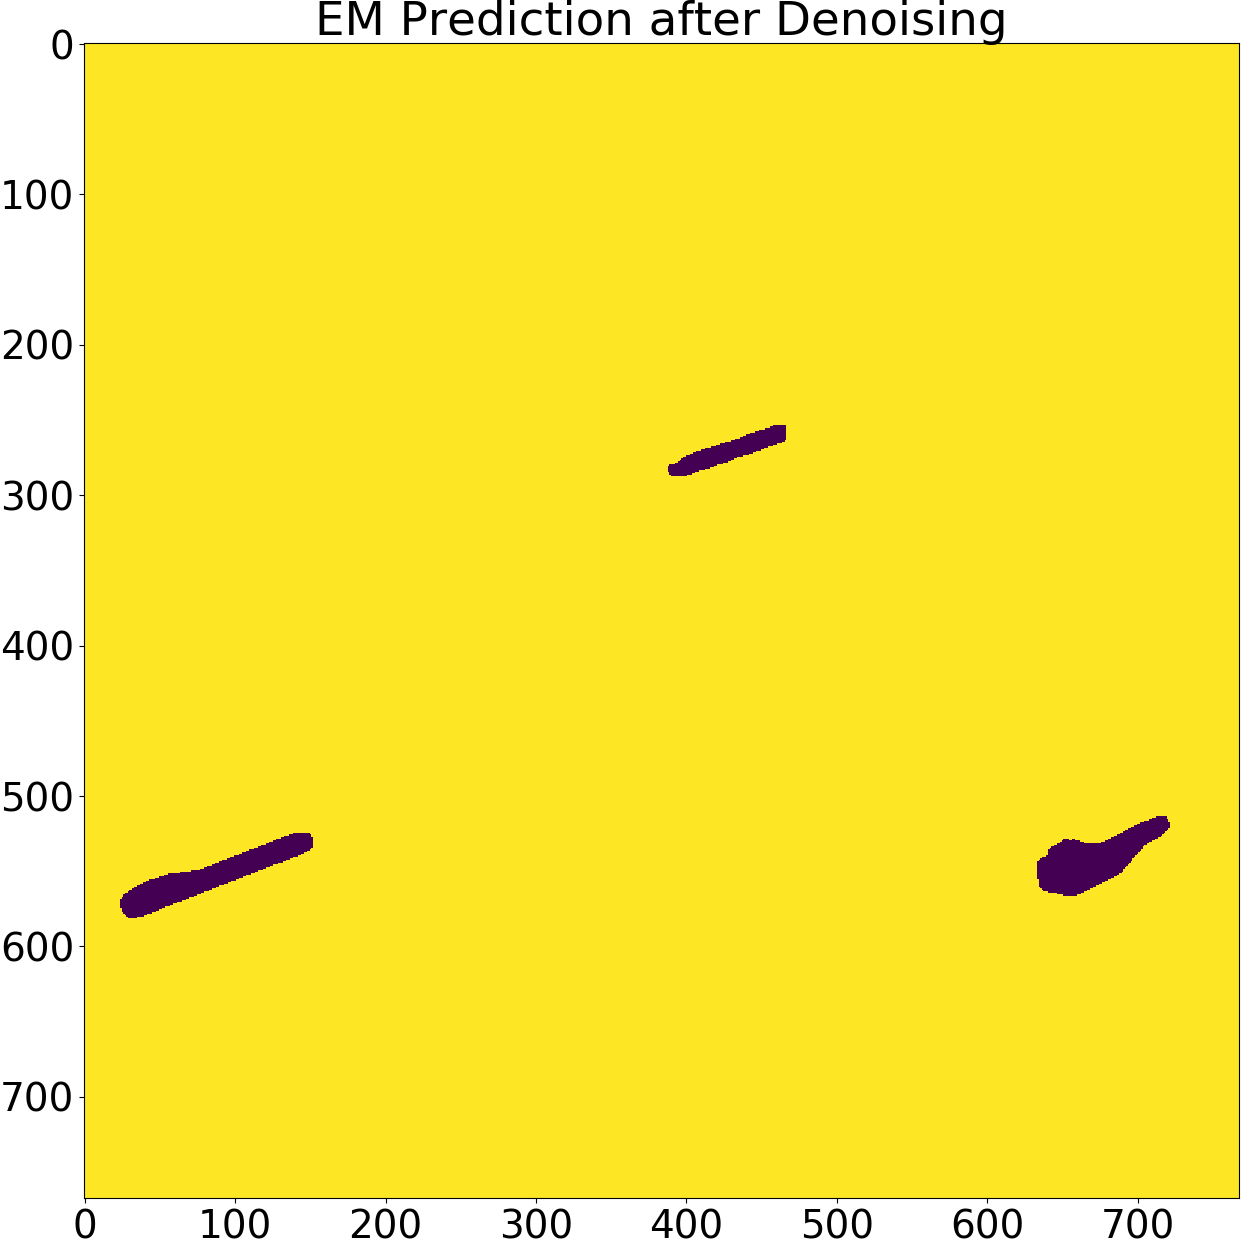
\includegraphics[width=0.45\textwidth]{Pictures/011Denoising.png}
	\caption{EM Result before and after denoising}
	\label{em_pic}
\end{figure}
\begin{figure}[H]
	\centering
	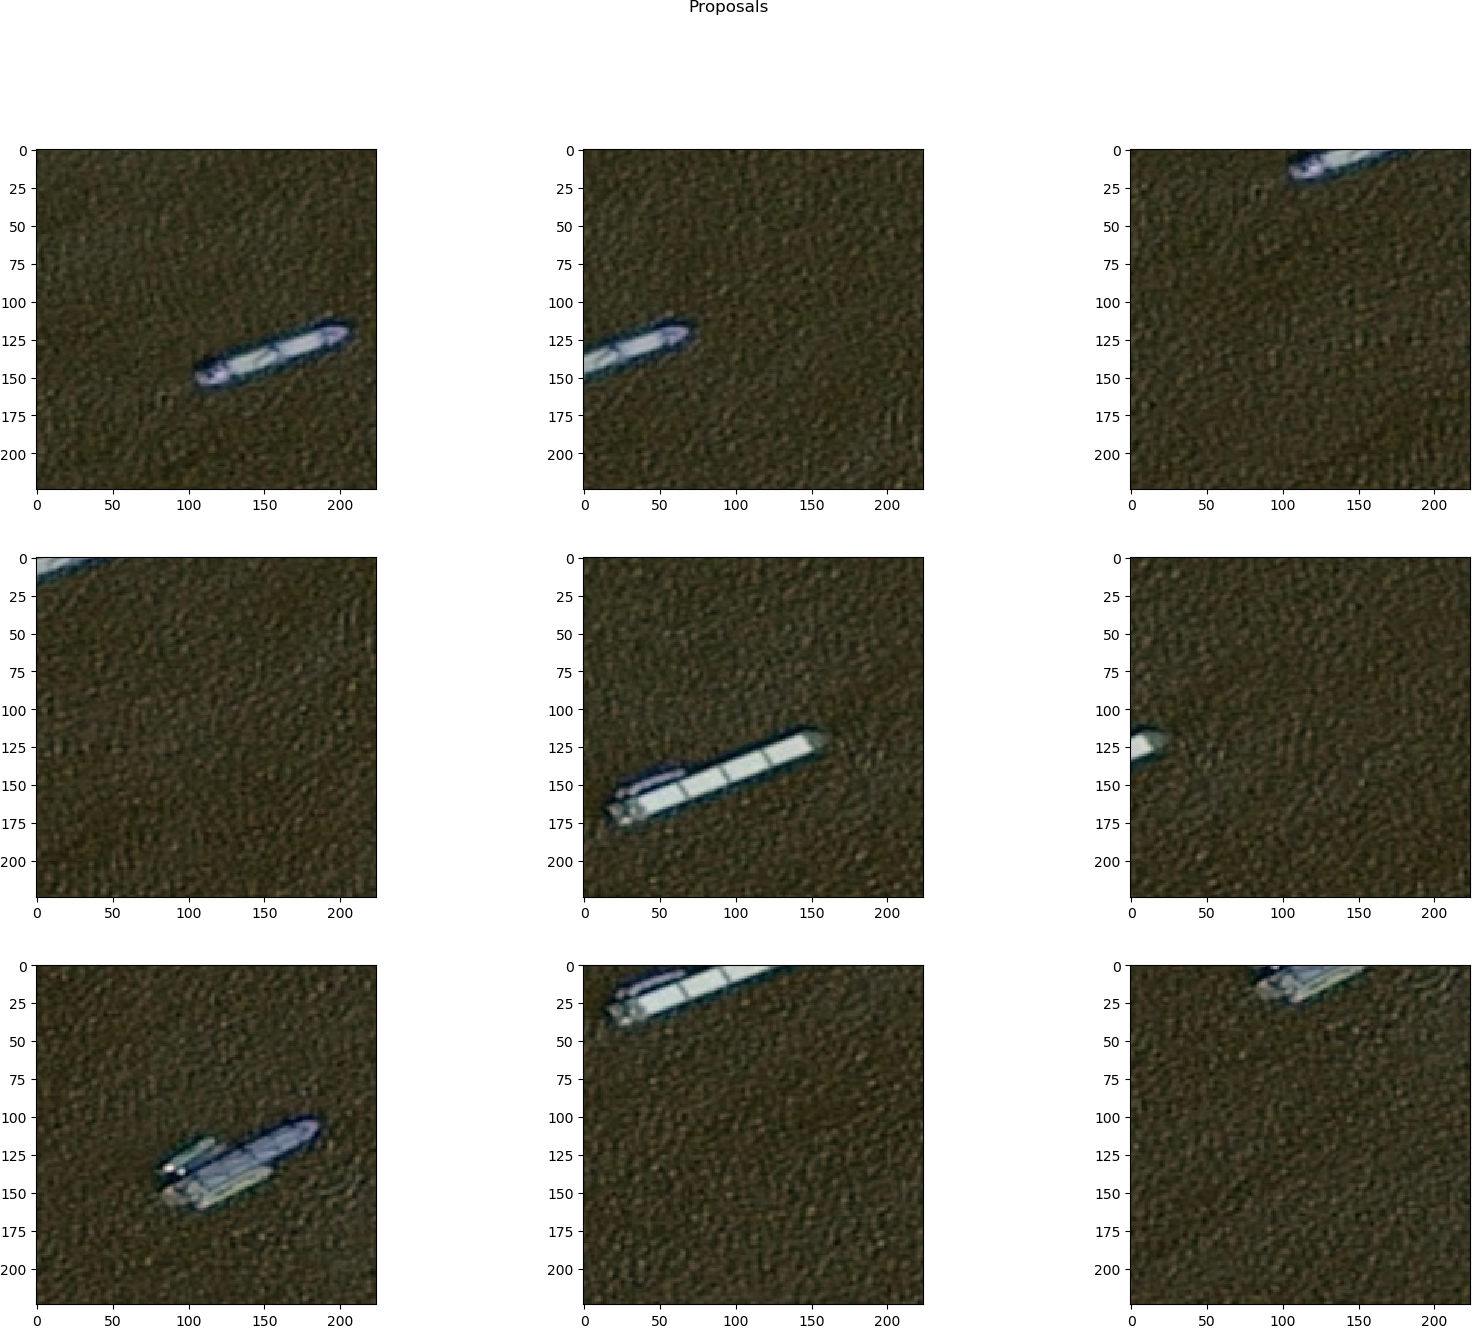
\includegraphics[height=0.6\textheight]{Pictures/011Proposals.png}\\
	\caption{9/25 proposed regions}
	\label{propose_pic}
\end{figure}
\begin{figure}[H]
	\centering
	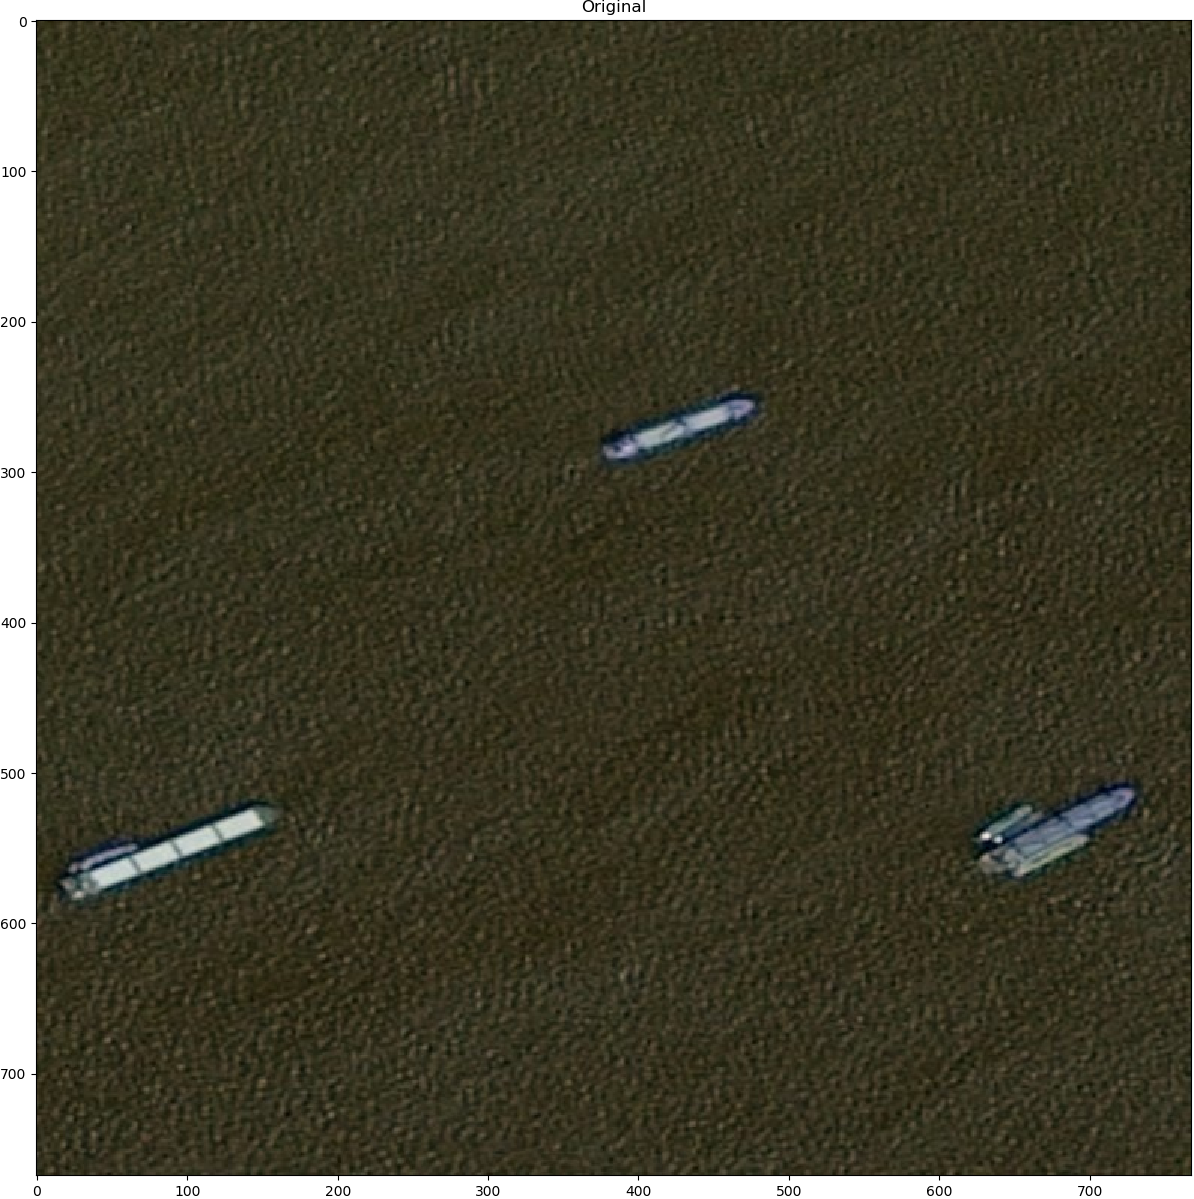
\includegraphics[width=0.45\textwidth]{Pictures/011Original.png}
	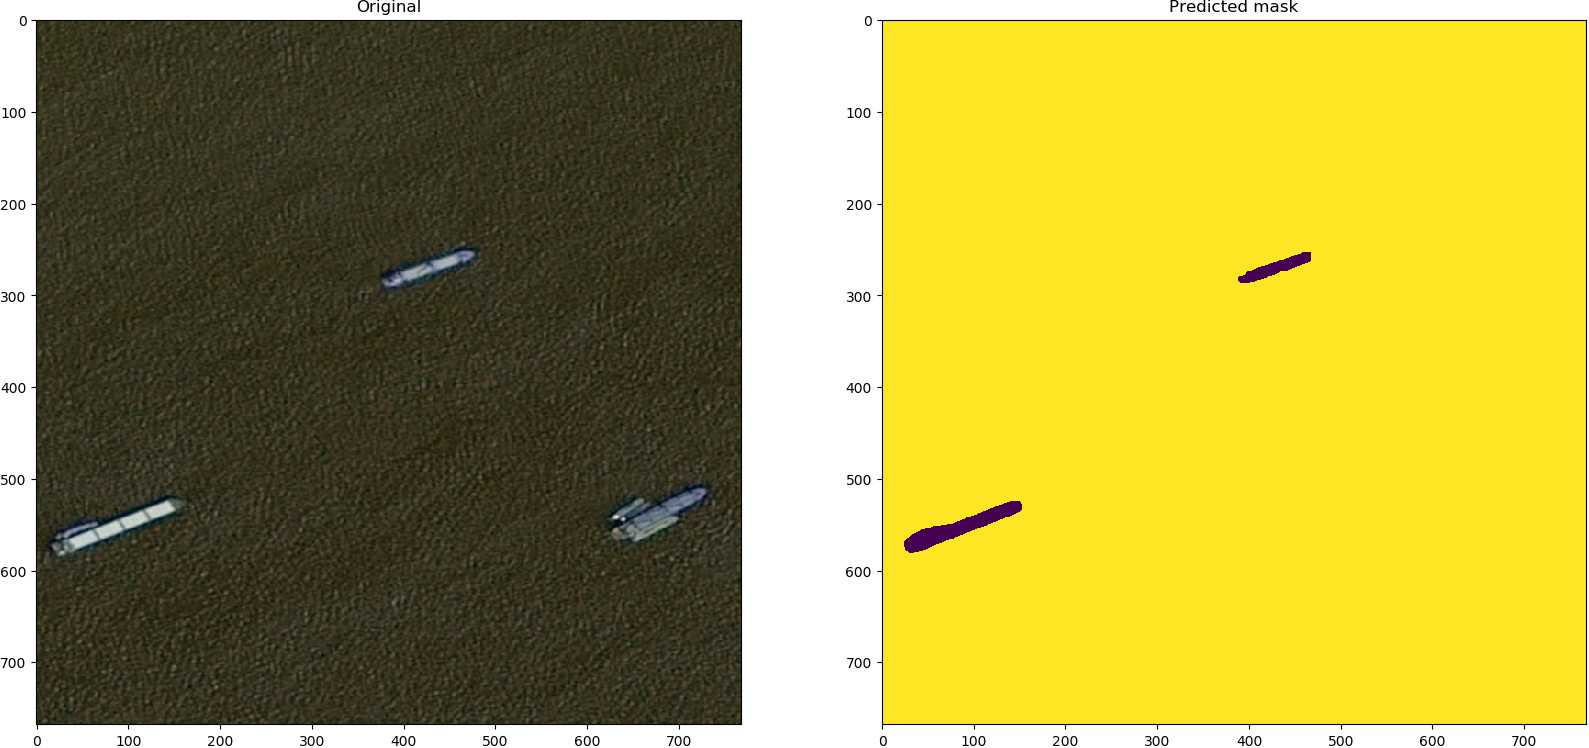
\includegraphics[width=0.45\textwidth]{Pictures/011FinalResult.png}
	\caption{Final Result}
	\label{final_result_pic}
\end{figure}


\section{U-Net Solution}
Another solution for solving the \textbf{(P3)}, was the usage of U-Nets \cite{Unet}. As show in \ref{UnetArch} the initial part of the classification stays the same as in the Region Proposal Solution. This solutions changes after the EM classification is finished. Instead of extracting proposed region for another classification, the pixels that were classified as background are turned black (Pixel Exclusion phase) in the original image, and afterwards the image is sent through a U-Net and a Gaussian smoothing for the final prediction.
\begin{figure}[h]
	\centering
	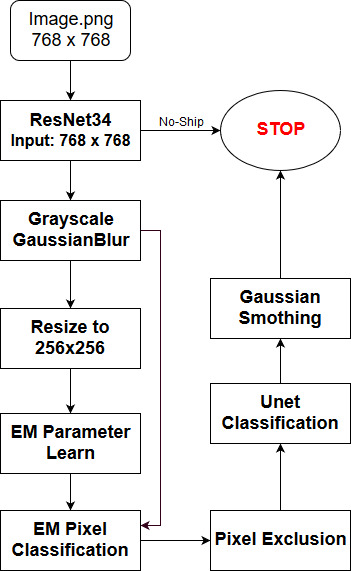
\includegraphics[width=0.5\textwidth]{Pictures/013UnetArchitecture.jpg}\\
	\caption{U-Net}
	\label{UnetArch}
\end{figure}

For the training of the U-net, a modified version of the $F_2$ score was used. Since inside a model training, the loss function must be minimized, and in the case of the $F_2$ score, a higher score means a better prediction, a loss function equal to $-F_2$ was used. The model was trained until the loss function reached the value of $-0.2$. On every training phase, the model pass thorough 10 epochs, and for each epoch 9 training steps were executed on the model. For every epoch 48 images were randomly selected from the training set.

\section{U-Net Example Run}
The following figures shows a picture in different stages of processing:
\begin{enumerate}
	\item \ref{orig_pic_unet} - as in the Region Proposal Solution the initial steps doesn't change. The picture is moved to grayscale, and the Gaussian filter is applied.
	\item \ref{em_pic_unet} - the classification result after the em algorithm where the yellow pixels are background, and the purple one are ships (left), and new image with the pixels classified as background are colored as black in the original image (right).
	\item \ref{final_result_pic_unet} - the final result compared to the initial picture. The final result is obtained by inserting the exclusion pixel image in the U-Net network.
\end{enumerate}
\begin{figure}[h]
	\centering
	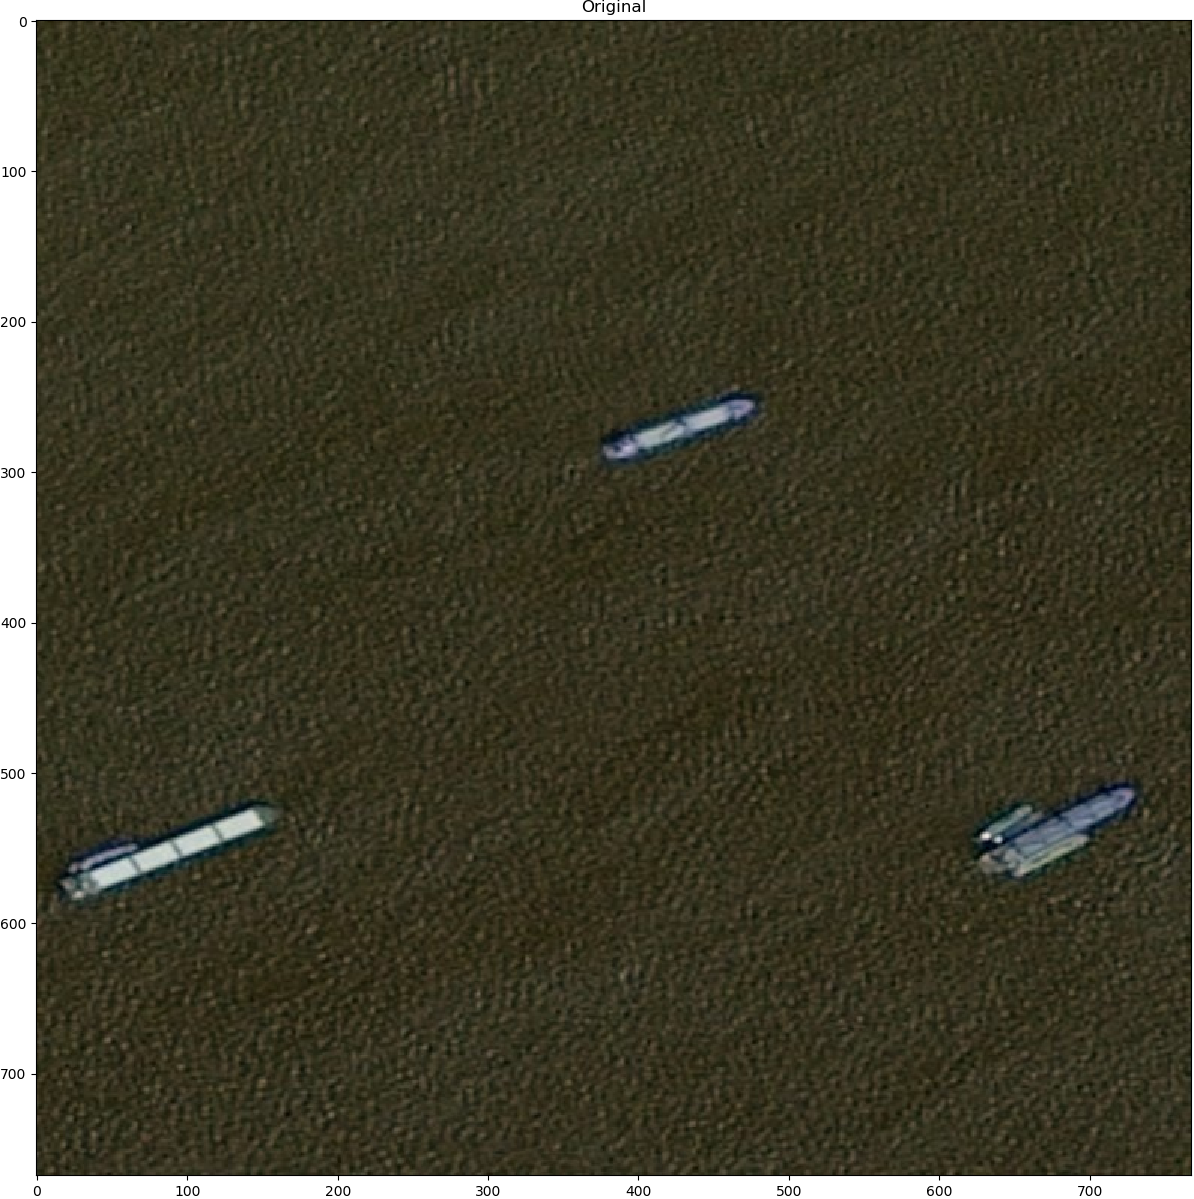
\includegraphics[width=0.45\textwidth]{Pictures/011Original.png}
	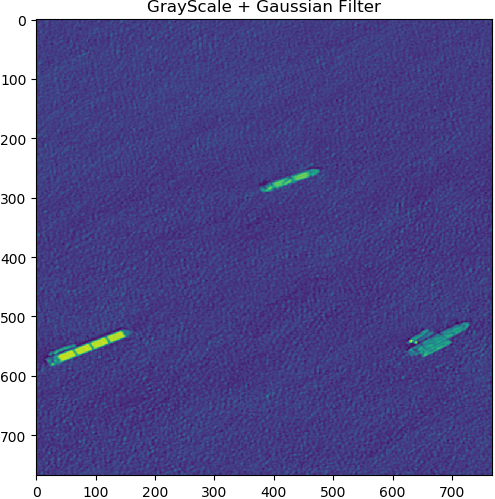
\includegraphics[width=0.45\textwidth]{Pictures/011GrayScale.png}
	\caption{Input/Original Picture, Grayscale and Gaussian Filtering}
	\label{orig_pic_unet}
\end{figure}
\begin{figure}[h] 
	\centering
	\includegraphics[width=0.45\textwidth]{Pictures/011EMPred.png}
	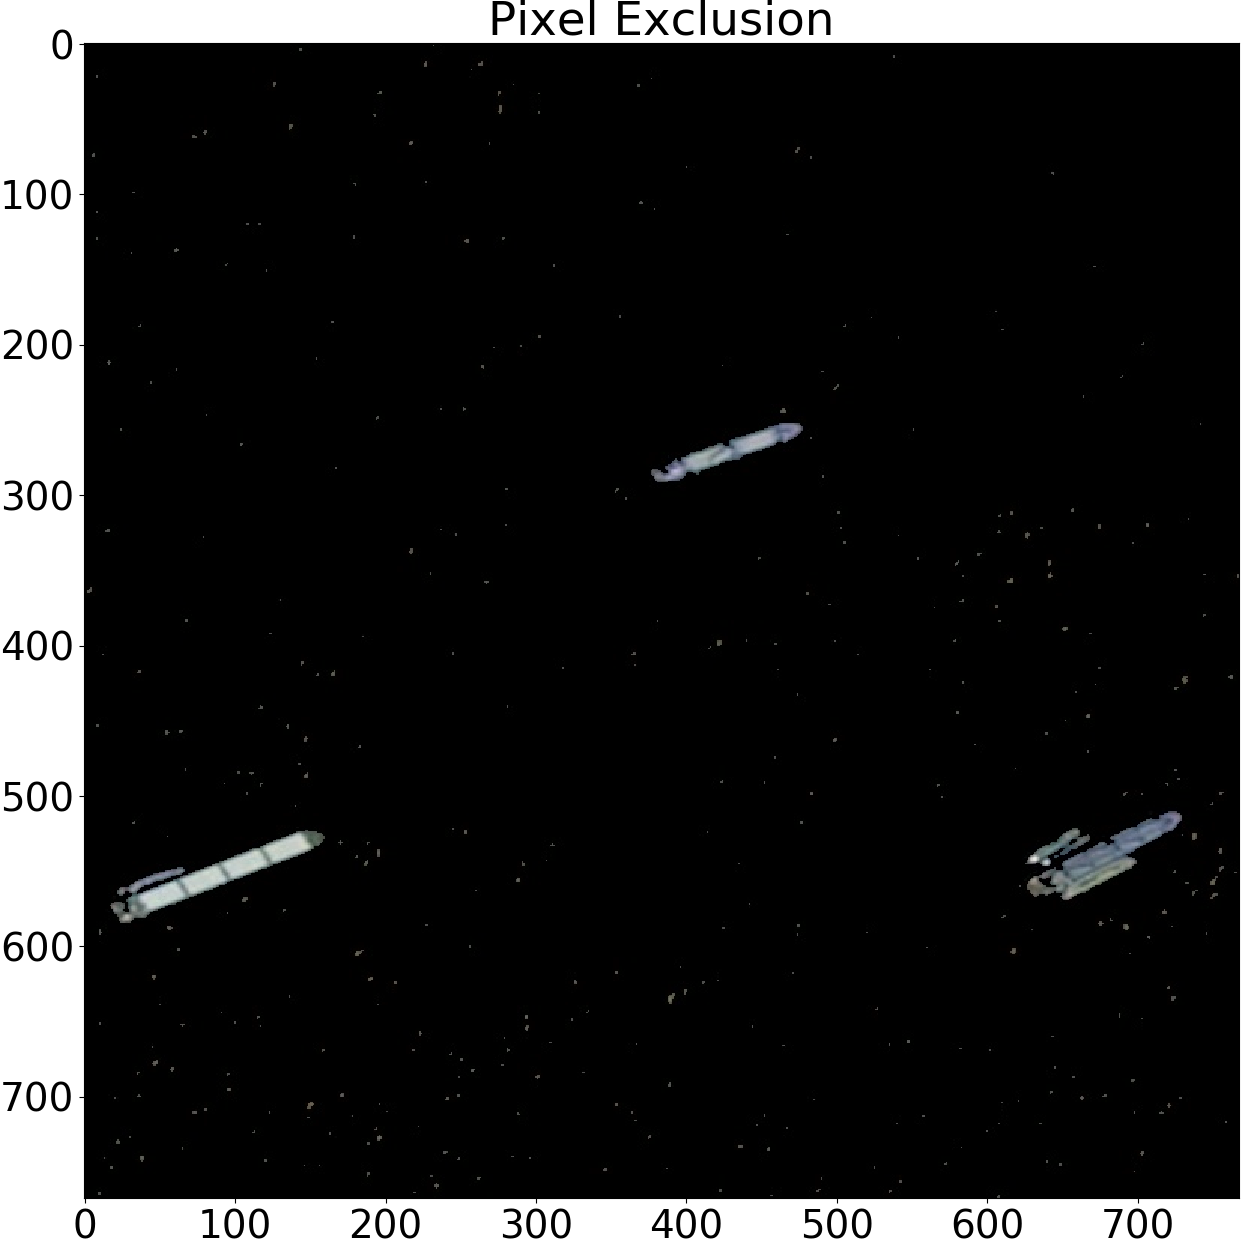
\includegraphics[width=0.45\textwidth]{Pictures/014PixelExclusion.png}
	\caption{EM Result and Pixel Exclusion}
	\label{em_pic_unet}
\end{figure}
\begin{figure}[h]
	\centering
	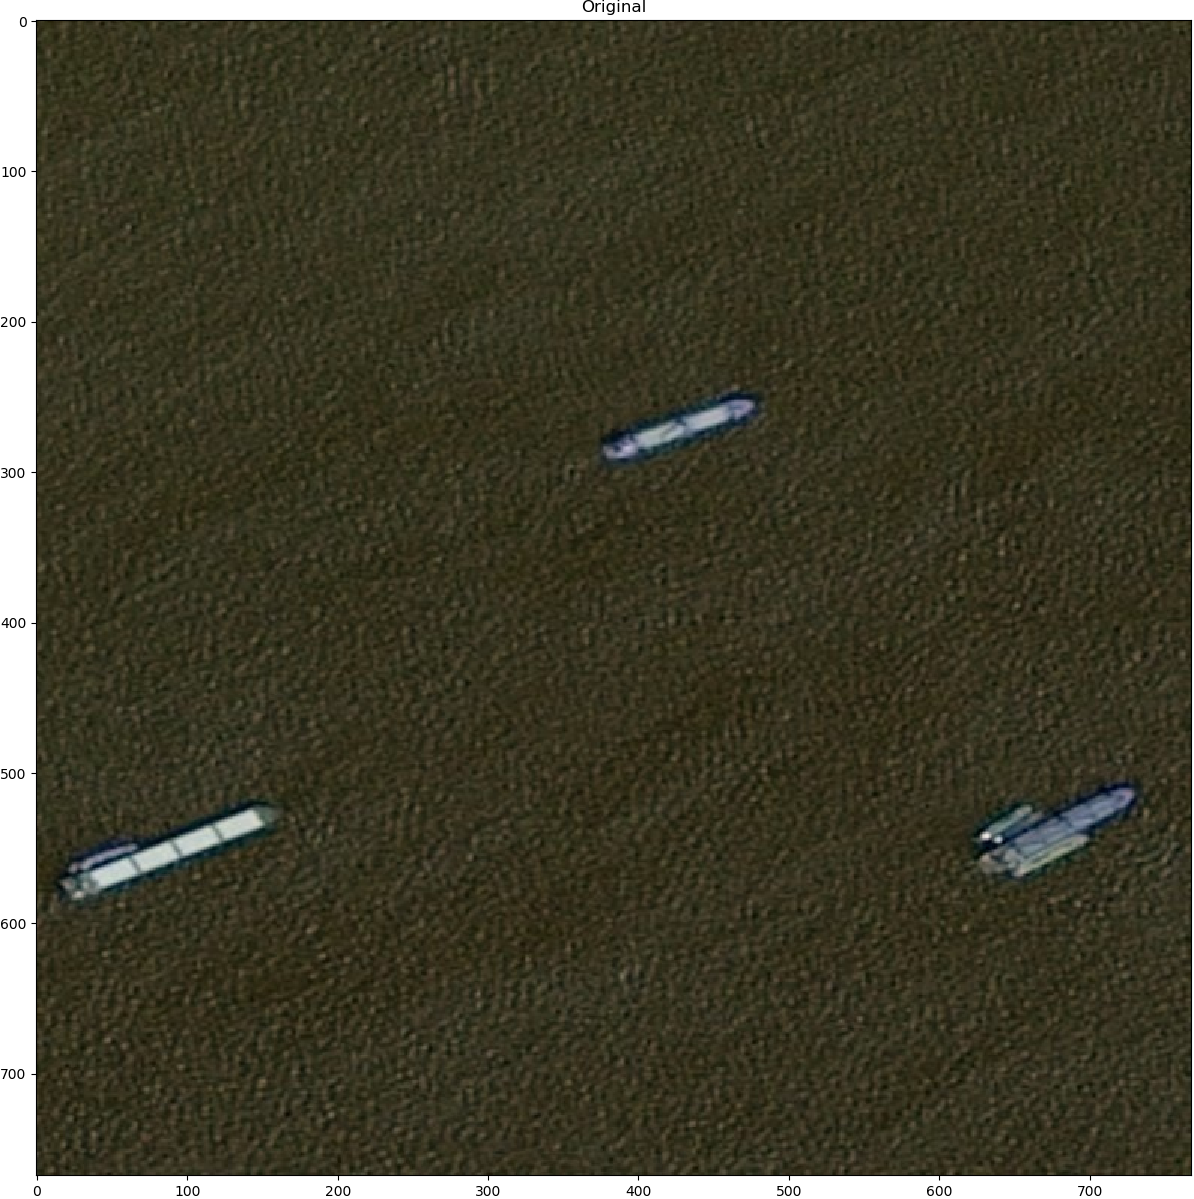
\includegraphics[width=0.45\textwidth]{Pictures/011Original.png}
	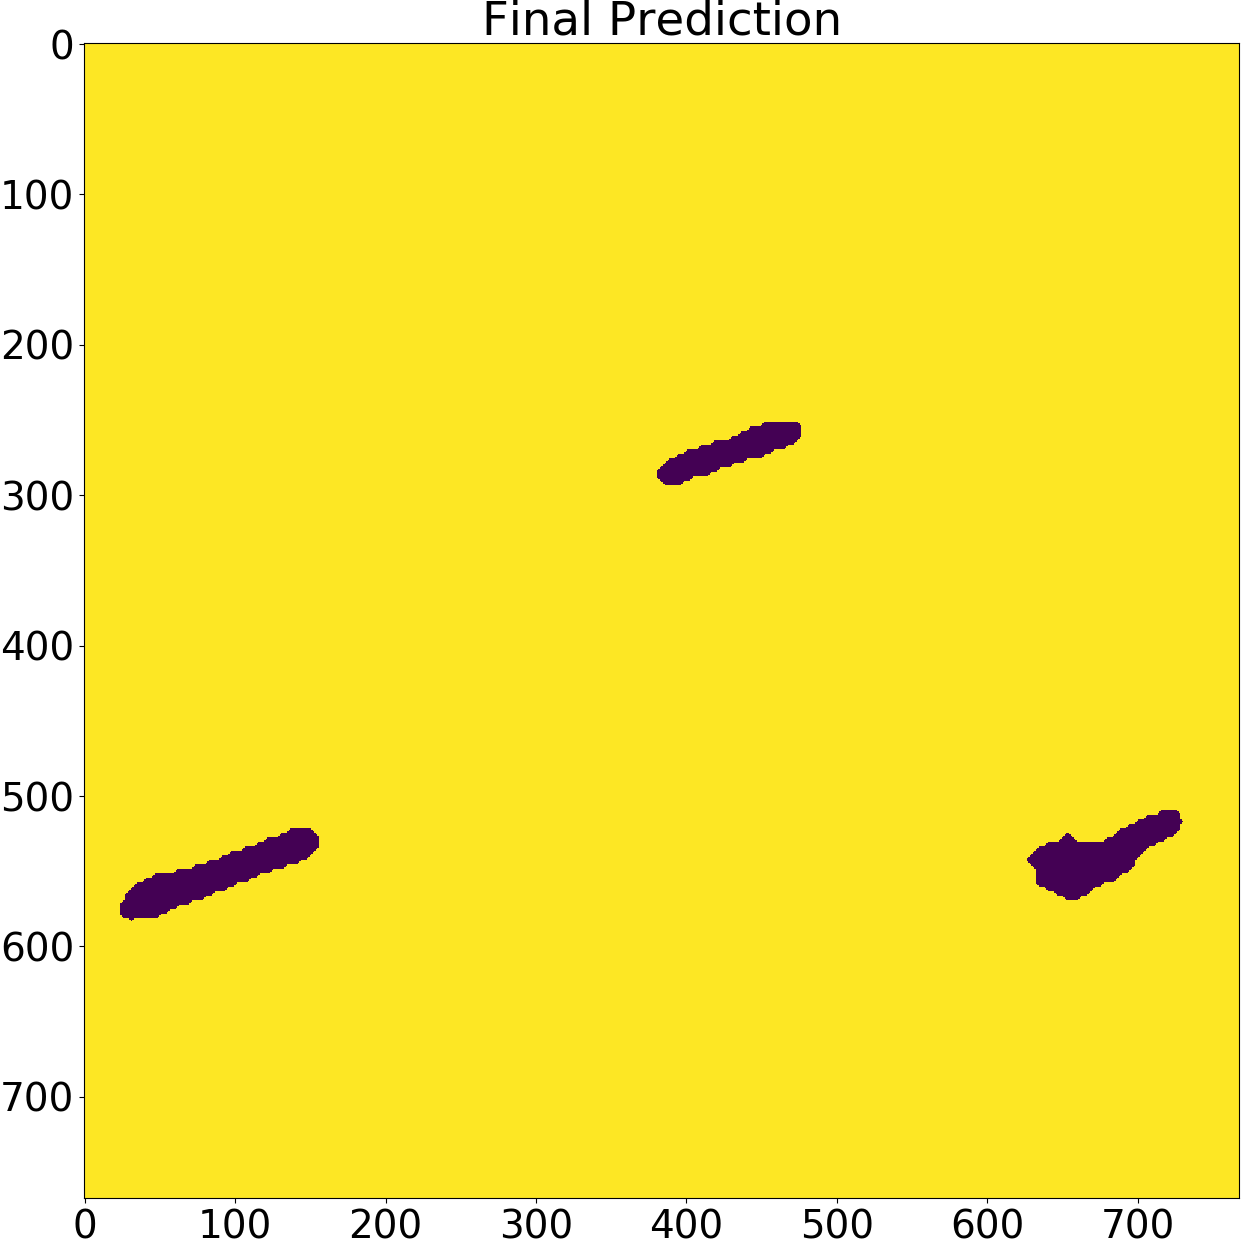
\includegraphics[width=0.45\textwidth]{Pictures/014FinalResult.png}
	\caption{Final Result}
	\label{final_result_pic_unet}
\end{figure} % Conslusion

\chapter{Conclusion and future work}
%\lhead{Introduction}
%\rhead{Radu-George Rusu}
Analyzing the result presented in the previous chapter we can see a pattern both on the real data sets and on the random ones. It is preferable to use either Hill Climbing or particle swarm optimization for this specific problem, because they yield better results both in terms of final output and also in terms of performances (time, CPU, memory). Also, from this results, we can say that it's more advantageous to use one those heuristics, rather than a deterministic algorithm. Although they may not yield the best result at every run, from a resource (time, memory) perspective, these heuristic are more convenient than a deterministic algorithm. In our concrete cases, on the real data sets, the exhaustive search algorithms took between 10 to 15 minutes to compute the final solution, while the heuristic ones were finished after 1 minute, with results similar to the exhaustive one.

Having this in mind, as a future point for this work, those algorithms can be ran on bigger datasets with more observations. The data sets used in this work are somehow of didactic size, and although the results are pretty good, we need a bigger scale to draw final results for real world data. Another point that can be used for future works is the usage of the optimization function. In this paper we used an estimator as the objective function instead of using a function that matches the data. A short example will be to use the sum squared errors function for a data set with a lot observations. We can split the initial data in training data (that will be used for running of the algorithm) and test data (that will be used for computing the objective function). In this way we will get solutions that are closer to the data that we used as input for the algorithm.

On the synthetic data, the results showed that this algorithms can fail in certain conditions. First of all, they were evaluated against a true solution, know before generating the input data, which is not necessarily the best solution in regards to AIC value. This can lead, in a future work, to usage of a different objective function (as described in the previous paragraph). To avoid the noise that we noticed with the 50 variables random data set, we can use other methods for variable selection (that can handle better that amount of noise), and chained it with the method presented here.

The last point of this work is the fact that the genetic algorithm behave quite poorly compared to the other 3 algorithms. This is mainly due to the representation of the solution and how the search space look like. For this algorithm 3 operators have been used, mutation, crossover and fortune wheel selection roulette. Although the first and the third one helps in optimizing this type of spaces, the crossover one actually adds more random solutions into the population, which explain in fact the slow convergence speed of this algorithm. As a future work the genetic algorithm can be run with other operators that are more suited for this type of solution spaces.

As final conclusions for this work, we can say that the Hill Climbing variations and Particle Swarm Optimization (as presented here) are a good choice when trying to solve this types of problems. The parameters can be tweaked to improve the performances of the algorithms, but this paper present a good starting point for new discoveries. % Conclusion

%\chapter{Conclusions}
\lhead{Conclusions}
\rhead{Radu-George Rusu}
This thesis presented a good starting point for using an unsupervised learning procedure, with the help of supervised learning, to detect ships from an aerial point of view. The EM algorithm works comparably well with both Residuals Networks and U-Net Network Architecture as shown in the Results chapter. Although, from the $F_2$ metric perspective the two solutions proposed didn't produce a large improvement over the base model, the expectation-maximization algorithm by itself, behaved well from a visual perspective, and can be used, in a practical environment, in conjunction with external help. The algorithm can be improved or even parallelized to reduce the execution time and to not give up accuracy.

The EM underlying model used is relatively simple, hence it can be improved with additional work. A first idea could be the usage of multi-level EM as shown in \cite{EMObjectConcealement}, or by using a different probability function (e.g. more than two Gaussians that generated the data). The biggest challenge that these solutions faced was the color similarity between ships and ports which gives us false negatives and a lower $F_2$ score. On the other hand, when the picture were taken "at sea", the algorithm produces good results. With this in mind, the algorithm in the actual form (or eventually improved forms) can be used on datasets that match the property of having two main colors scheme inside them.
 % Results and Discussion

%\input{Chapters/Chapter7} % Conclusion

%% ----------------------------------------------------------------
% Now begin the Appendices, including them as separate files

\addtocontents{toc}{\vspace{2em}} % Add a gap in the Contents, for aesthetics

\appendix % Cue to tell LaTeX that the following 'chapters' are Appendices

%\input{Appendices/AppendixA}	% Appendix Title

%\input{Appendices/AppendixB} % Appendix Title

%\input{Appendices/AppendixC} % Appendix Title

\addtocontents{toc}{\vspace{2em}}  % Add a gap in the Contents, for aesthetics
\backmatter

%% ----------------------------------------------------------------
\label{Bibliography}
\lhead{\emph{Bibliography}}  % Change the left side page header to "Bibliography"
\bibliographystyle{unsrtnat}  % Use the "unsrtnat" BibTeX style for formatting the Bibliography
\bibliography{Bibliography}  % The references (bibliography) information are stored in the file named "Bibliography.bib"

\end{document}  % The End
%% ----------------------------------------------------------------